%\documentclass{book}\usepackage{sjtfonts}\usepackage{includegraphics}\usepackage{alltt}\usepackage{latexsym}
%\usepackage{array}
%\begin{document}\input{defs0}%		miradefs.tex 		    June 1994

% opening and closing a quoted Miranda section

\newcommand{\mira}{\noindent\hrulefill\nopagebreak\so}
\newcommand{\arim}{\nopagebreak\st\hrulefill\\}

% backslash in the Miranda environment
% Only feasible approach is to use \verb+\+
% in line!

%\newcommand{\bs}{$\mi\backslash\!\!$}
%\newcommand{\lbs}{\mbox{\verb+\+}}

% ignoring part of the input

\newcommand{\ignore}[1]{}

% a blank line in a Miranda section

\newcommand{\bl}{\mbox{\ }}

% Signalling a diffculty.

\definecolor{light-gray}{gray}{0.95}

\newcommand{\beware}[2]
 {\medskip\noindent\colorbox{light-gray}{\parbox{\textwidth}
 {\mbox{\large\textbf{#1}} \medskip\noindent\\ #2}\medskip\noindent}}

% Subscripting in Miranda text
\newcommand{\subscr}[2]{\mbox{${\mbox{\texttt{#1}}}_{\mbox{\texttt{#2}}}$}}

%\newcommand{\subscr}[2]{\mbox{${\mbox{\mi #1}}_{\mbox{\smtt #2}}$}}
\newcommand{\aone}{\subscr{a}{1}}
\newcommand{\atwo}{\subscr{a}{2}}
\newcommand{\ak}{\subscr{a}{k}}

\newcommand{\aoneone}{\subscr{a}{1,1}}

\newcommand{\eone}{\subscr{e}{1}}
\newcommand{\etwo}{\subscr{e}{2}}
\newcommand{\ei}{\subscr{e}{i}}
\newcommand{\er}{\subscr{e}{r}}

\newcommand{\fone}{\subscr{f}{1}}
\newcommand{\fl}{\subscr{f}{l}}

\newcommand{\gone}{\subscr{g}{1}}
\newcommand{\gtwo}{\subscr{g}{2}}
\newcommand{\gi}{\subscr{g}{i}}
\newcommand{\gr}{\subscr{g}{r}}

\newcommand{\hone}{\subscr{h}{1}}
\newcommand{\hl}{\subscr{h}{l}}

\newcommand{\pone}{\subscr{p}{1}}
\newcommand{\ptwo}{\subscr{p}{2}}
\newcommand{\pk}{\subscr{p}{k}}

\newcommand{\qone}{\subscr{q}{1}}
\newcommand{\qtwo}{\subscr{q}{2}}
\newcommand{\qk}{\subscr{q}{k}}

\newcommand{\rone}{\subscr{r}{1}}
\newcommand{\rtwo}{\subscr{r}{2}}

\newcommand{\tone}{\subscr{t}{1}}
\newcommand{\ttwo}{\subscr{t}{2}}
\newcommand{\tn}{\subscr{t}{n}}

\newcommand{\vone}{\subscr{v}{1}}
\newcommand{\vtwo}{\subscr{v}{2}}
\newcommand{\vn}{\subscr{v}{n}}

% for regular expressions

\newcommand{\stone}{\subscr{st}{1}}
\newcommand{\sttwo}{\subscr{st}{2}}
\newcommand{\stn}{\subscr{st}{n}}
\newcommand{\rthree}{\subscr{r}{3}}

\newcommand{\eps}{$\varepsilon$}
\newcommand{\trans}[1]{\stackrel{\mbox{\tt #1}}{\longrightarrow}}



% superscript in Miranda text

\newcommand{\superscr}[2]{\mbox{${\mbox{\mi #1}}^{\mbox{\smtt #2}}$}}

% Not equals in Miranda text

\newcommand{\noteq}{\makebox[0pt][l]{=}/}
\newcommand{\overslash}{\makebox[0pt][l]{/}}

% Definitions in complexity chapter

\newfont{\oldSym}{cmsy10}
\newcommand{\Th}{\boldmath$\oldSym\Theta$}
\newcommand{\pow}[1]{\^{}#1}
\newcommand{\leqq}{$\leq$}
\newcommand{\geqq}{$\geq$}
\newcommand{\lll}{$\ll$}
\newcommand{\eqq}{$\equiv$}
\newcommand{\ltwo}{\subscr{log}{2}}

% Indexing

\newcommand{\minx}[1]{\index{#1@{\ttfamily{}#1}}}
\setcounter{chapter}{14}\setcounter{page}{269}

\chapter{Case study: Huffman codes}
\chapstart
\label{codes}
\index{Huffman codes|(}
\index{case studies!Huffman codes|see{Huffman codes}}

We use the case study in this chapter as a vehicle to illustrate many of the
features of the previous chapters -- polymorphism, algebraic types and
program design -- and to illustrate the module system of Haskell,
which is discussed first.


\section{Modules in Haskell}
\index{modules|(}

As we first saw in Section \ref{introModules}, a module
consists of a number of definitions of types, functions and so on, with a
clearly defined \emph{interface} stating what the module \texttt{exports} to
other modules which use or \texttt{import} it. We also saw in Section \ref{HaskellLibs} that module names can be composite, as in \texttt{Data.Bits}, taking the form of hierarchical names.

\medskip
\noindent
Using modules to structure a large program has a number of advantages.
\begin{titemize}
\item Parts of the system can be built separately from each other. Suppose we
want to monitor traffic on a network: one module might produce the statistics,
while another displays them in a suitable form.
If we agree which statistics are to
be presented (their type etc.), that is we agree the interface, then
development of the two parts of the system can go on independently.
\item Parts of a system can be compiled separately; this is a great advantage
for a system of any complexity.
\item Libraries of components can be reused, by importing the appropriate
modules containing them.
\end{titemize}
In the definition of Haskell 2010, there is no identification
between modules and files. Nonetheless, we
choose here to write one module per file, and indeed this is required by GHC.

Now we look at the details of Haskell modules, before giving our case study which
exhibits the system in action.

\subsection*{Module headers}

Each module is named, so an example named \texttt{Ant} might be
\begin{alltt}
module Ant where\minx{module}\minx{Ant}

data Ants  = ...
anteater x = ...
\end{alltt}
Note that the definitions all begin in the column under the keyword
\texttt{module}; it is safest to make this the leftmost column of the
file.


We also assume that a module \texttt{Foo} will live in the file \texttt{Foo.hs}; GHC allows module and file names to be different, but we recommend that you keep them the same. \index{conventions!module file names}

\subsection*{Importing a module}

The basic operation on modules is to \texttt{import} one into another, so in
defining \texttt{Bee} we might say
\begin{alltt}
module Bee where\minx{Bee}

import Ant\minx{import}

beeKeeper = ...
\end{alltt}
This means that the \textbf{visible} definitions from \texttt{Ant}
can be used in 
\texttt{Bee}. By default the visible definitions in\index{visibility of
definitions}\index{definition!visibility of}
a module are those which appear in the module itself. If we define
\begin{alltt}
module Cow where\minx{Cow}

import Bee
\end{alltt}
the definitions of \texttt{Ants} and \texttt{anteater} will not be visible in 
\texttt{Cow}. They can be made visible either by importing \texttt{Ant} explicitly,
or by using the export controls
discussed below to modify exactly what is exported from \texttt{Bee}.


\subsection*{Export controls}
\index{export}

As we explained when \texttt{import} was introduced,
the default is that all top-level definitions of a
module are exported. 
\begin{titemize}
\item This may be too much: we might wish not to export some
auxiliary functions, such as the \texttt{shunt} function below
\begin{alltt}
reverse :: [a] -> [a]
reverse = shunt []

shunt :: [a] -> [a] -> [a]
shunt ys []     = ys
shunt ys (x:xs) = shunt (x:ys) xs
\end{alltt}
since its only role is in defining the \texttt{reverse} function.
\item On the other hand, it might be too little: we perhaps want
to export some of the definitions we imported from other modules. The modules
\texttt{Ant}, \texttt{Bee} and \texttt{Cow} above provide an example of this.
\end{titemize}
We can control what is exported by following the name of the module with a
list of what is to be exported. For instance, we say in the case of \texttt{Bee}
\begin{alltt}
module Bee ( beeKeeper, Ants(..), anteater ) where ...\minx{module}\index{modules!export list}
\end{alltt}
The list contains names of defined objects, such as \texttt{beeKeeper}, and also
\texttt{data} types like \texttt{Ants}.
In the latter case we follow the type name with \texttt{(..)} to indicate
that the constructors of the type are exported with the type
itself; if this is omitted, then the type acts like an \textbf{abstract
data type},\index{abstract data type} which we investigate further in the next chapter. The
\texttt{(..)} is\minx{(..)}
not necessary for a \texttt{type} definition.

Such a list works on a definition-by-definition basis; we can also state that
all the definitions in a module are to be exported, as in
\begin{alltt}
module Bee ( beeKeeper, module Ant ) where ...
\end{alltt}
or equivalently
\begin{alltt}
module Bee ( module Bee , module Ant ) where ...
\end{alltt}
where preceding the name of a module by the keyword \texttt{module} 
is shorthand for
all the names defined within the module. The simple header
\begin{alltt}
module Fish where
\end{alltt}
is therefore equivalent to 
\begin{alltt}
module Fish ( module Fish ) where
\end{alltt}


\beware{The \texttt{Main} module}{
Each system of modules should contain a top-level
module called \texttt{Main}, which gives a
definition to the name \texttt{main}. In a compiled system, this is
the\minx{Main}\minx{main}
expression which is evaluated when the compiled code is run. In an
interpreter like GHCi, where we can run code in any module, it is of less significance. 

\medskip
A module 
without a header is treated as though it contains the header 
\begin{alltt}
module Main(main) where
\end{alltt} 
}


\subsection*{Import controls}
\minx{import}

We can control how objects are to be imported, just as we can control their
export. We do this by following the \texttt{import} statement with a list of
objects, types or classes. For instance, if we choose not to import 
\texttt{anteater} from \texttt{Ant} we can write

\index{modules!import list}\begin{alltt}
import Ant ( Ants(..) )
\end{alltt}
stating that we want just the type \texttt{Ants}; we can alternatively say which
names we wish to {\em hide}:
\begin{alltt} 
import Ant hiding ( anteater )\minx{hiding}
\end{alltt}
Suppose that in our module we have a definition of \texttt{bear}, and also there
is an object named \texttt{bear} in the module \texttt{Ant}. How can we gain access
to {\em both\/} definitions? The answer is that we use the \textbf{qualified}
name \texttt{Ant.bear} for the imported object, reserving \texttt{bear} for the
locally defined one.\index{name!qualified} 

A qualified name is built from the
name of a module and the name of an object in that module, separated by a full
stop. Note that there should be {\em no\/}
white space between the `\texttt{.}' and the
two names, so as to avoid confusion with the composition operator. 
To use qualified names we should make the import like this:
\begin{alltt}
import qualified Ant\minx{qualified}
\end{alltt}
In the qualified case we can also state which particular items are to be
imported or hidden, just as in the unqualified case above. It is
possible to use a local name for an imported module, as in
\index{modules!local name on \texttt{import}}\minx{=}
\begin{alltt}
import Insect as Ant
\end{alltt}
which gives the local name \texttt{Ant} to the imported module
\texttt{Insect}.


\beware{Qualified and unqualified names}{\index{qualified names}
When a file is imported unqualified, that is without the \texttt{qualified} keyword, it is still possible to used qualified naming, so after importing \texttt{Ant} we can use both \texttt{anteater} and \texttt{Ant.anteater} to name the anteater function defined in that module. 

\medskip
On the other hand, if a file is imported \texttt{qualified} then only qualified names can be used. This note also applies when a module is given a local name, as in 
\begin{alltt}
import qualified Ant as Insect
\end{alltt}
after which the \texttt{anteater} function can only be invoked using \texttt{Insect.anteater}.

\medskip
One thing you need to be careful about is that you can't use a qualified name for a function \emph{within the function definition itself}, but only outside that definition.}




\subsection*{The standard \texttt{Prelude}}

The standard \texttt{Prelude} is implicitly imported into
every module. If we wish we can modify this import, perhaps
\texttt{hiding} one or more bindings thus
\begin{alltt}\minx{Prelude.hs}
module Eagle where

import Prelude hiding (words)
\end{alltt}
so that we can give our own definition of the name \texttt{words}. If we
import \texttt{Eagle}
into another module, this module will also have explicitly to hide the import of
\texttt{words} from the \texttt{Prelude} if conflicting definitions are to be avoided, and
so we see that a re-definition of a \texttt{Prelude} function cannot be
done `invisibly', as it were. 

If we also wish to have access to the original definition of \texttt{words}
we can make a qualified import of the prelude,
\begin{alltt}
import qualified Prelude
\end{alltt}
and use the original \texttt{words} by writing its qualified name
\texttt{Prelude.words}.

\subsection*{Further details}

Further information about the Haskell module system can be found
in the language report
\cite{haskell2010};
note that some of the details will be different in particular
implementations.



\begin{exercises}

\item
Can you get the effect of export controls using \texttt{import}? Can you get
the effect of the qualifications of \texttt{import} using export controls?
Discuss why both directives are included in the language.

\item
Explain why you think it is the default that \texttt{import}ed definitions
are not themselves exported.

\item
It is proposed to add the following option to the \texttt{module} export
control and the \texttt{import} statement.
If the item \texttt{-module Dog}
appears, then none of the definitions in the module \texttt{Dog} is exported or
imported. Discuss the advantages and disadvantages of this proposal. How would
you achieve the effect of this feature in the existing Haskell module system?
\index{modules|)}
\end{exercises}

\section{Modular design}
\index{design!modules}

Any computer system which is used seriously will be modified during its
lifetime, either by the person or team who wrote it, or more likely by
others.
For this reason, all systems should be designed with {\em change\/} in mind. 

We
mentioned this earlier when we said that systems should be \textbf{documented}, with
types given to all top-level definitions, and comments accompanying each
script and substantial definition. Another useful form of description is to
link each definition with proofs which concern it; if we know some of the
logical properties of a function, we have a more solid conception of its
purpose.\index{proof!as documentation}

Documentation \index{documentation}makes a script easier to understand, and therefore change, but
we can give \textbf{structure} to a collection of definitions if they are split
among modules or scripts, each script concerning a separate part of
the overall system. The directives which link the files tell us how the parts
of the system fit together. If we want to modify a particular part of a
system, we should therefore be able to modify a single module (at least
initially), rather than starting by modifying the whole of the
system as a single unit.

How should we begin to design a system as a collection of modules? The pieces
of advice which follow are aimed to make modification as straightforward as
possible.
\begin{titemize}
\item Each module should have a \textbf{clearly identified role}.
\item Each module should do \textbf{one} thing only. If a module has two
separate purposes, these should be split between two separate modules. The
chance of a change to one affecting the other is thereby reduced.  
\item Each part of the system should be performed by one module: each module
should do one thing completely; it should be self-contained, in other
words. If performing one part of the whole is split between two modules, then
either their code should be merged, or there should be a module defined with
the single purpose of bringing the two components together. 
\item Each module should export only what is necessary. It is then
clearer what the effect of an \texttt{import} is: precisely the
functions which are needed are imported. This process is often called
\textbf{information hiding}\index{information hiding} 
in software engineering, which is itself the general
study of principles for programming in the large.
\item Modules should be \textbf{small}. As a rule of thumb, no module should be
larger than can be printed on two or three sides of paper.  
\end{titemize}
We
have also mentioned design for \textbf{reuse}\index{reuse}, particularly in the context of
polymorphic types and higher-order functions. The module will be the unit of
reuse, and a library will be accessed by means
of an \texttt{import} statement. Similar principles apply to the design of
libraries. Each library should have a clearly defined purpose, like
implementing a type together with basic operations over the type. In addition,
we can say that  
\begin{titemize}
\item on including a general-purpose module, it
is possible to suppress the definitions which are not used;
\item a qualified \texttt{import} can be used to avoid the name-clashes
which can often occur: despite the (infinite) choice of names for functions,
in practice we tend to choose from a very small subset! 
\end{titemize}
The advice here might seem dry -- what has
been said is illustrated in the case study which follows. In the next chapter we will return
to the idea of information hiding when we meet abstract data types. In the
remainder of this chapter we examine the case study of Huffman coding, the 
foundations of which we explore now.



\section{Coding and decoding}
\label{codeIntro}
\index{coding|(}

Electronic messages of various kinds are sent between machines and people by
the billion each day. Such messages are usually sent as sequences of binary
`bits'. For the transmission to be swift, the messages need to be coded
as efficiently as possible. The area we explore here is how to build codes --
translations of characters into sequences of bits -- which produce 
messages as compact as possible.

Trees \index{coding!tree}
can be used to code and decode messages. Consider as an example the tree
\begin{center}
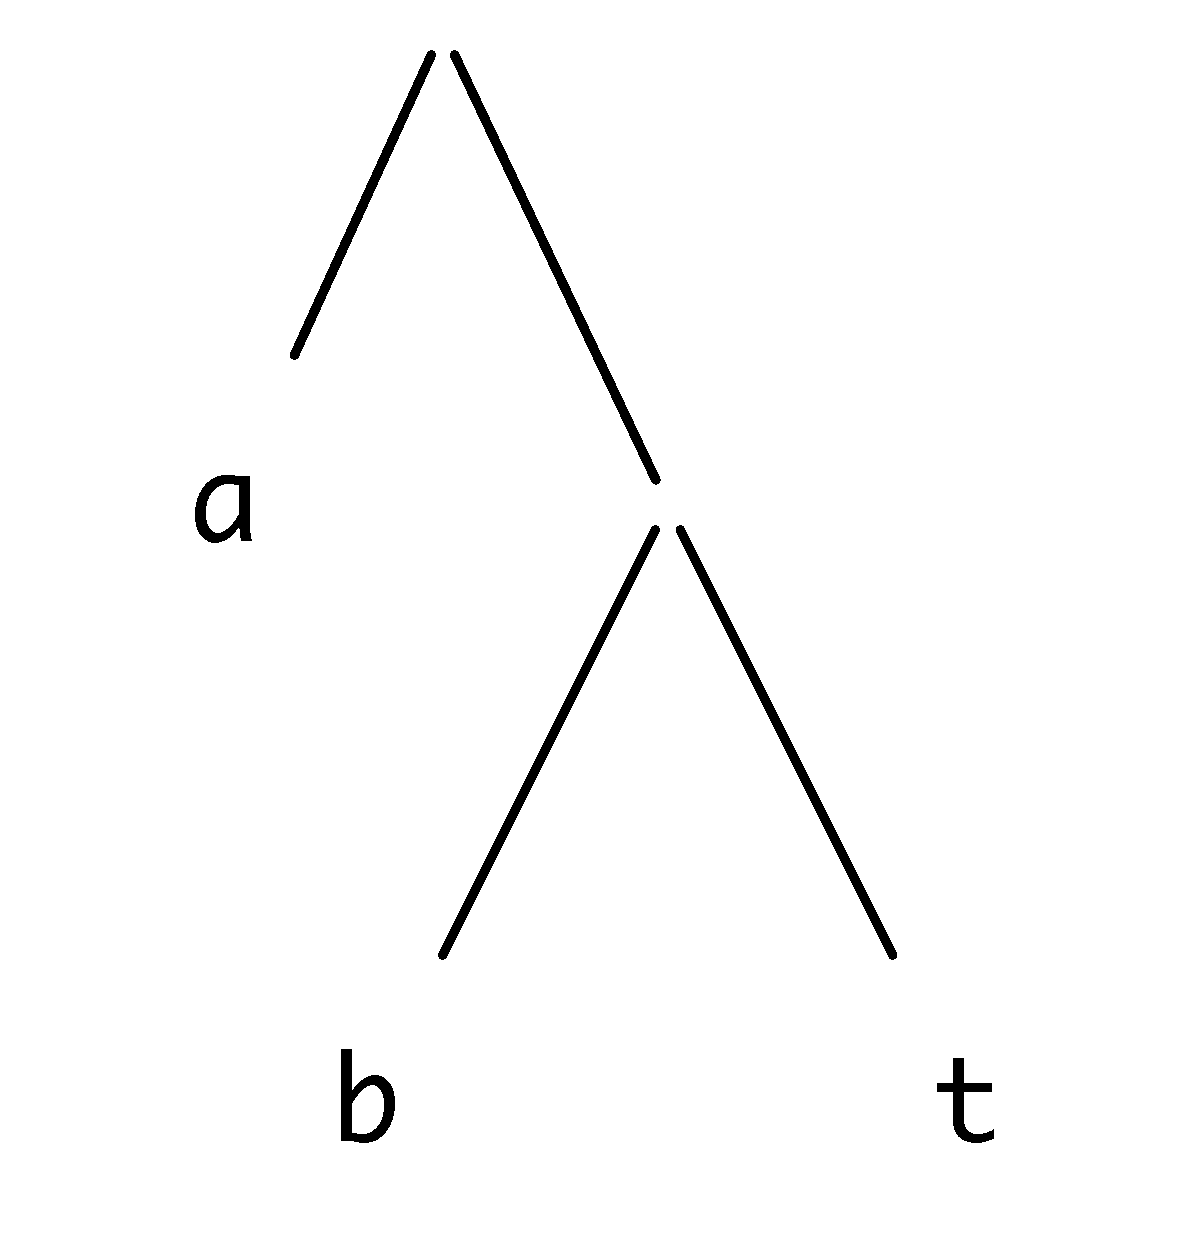
\includegraphics[width=1in]{Pictures/Huffman1.pdf}
\end{center}
We can see this as giving codes for the letters \texttt{a}, \texttt{b} and \texttt{t}
by looking at the \textbf{routes} taken to reach the letters. For example, to
get to \texttt{b}, we go {\em right\/} at the top node, and {\em left\/} at the
next: 
\begin{center}
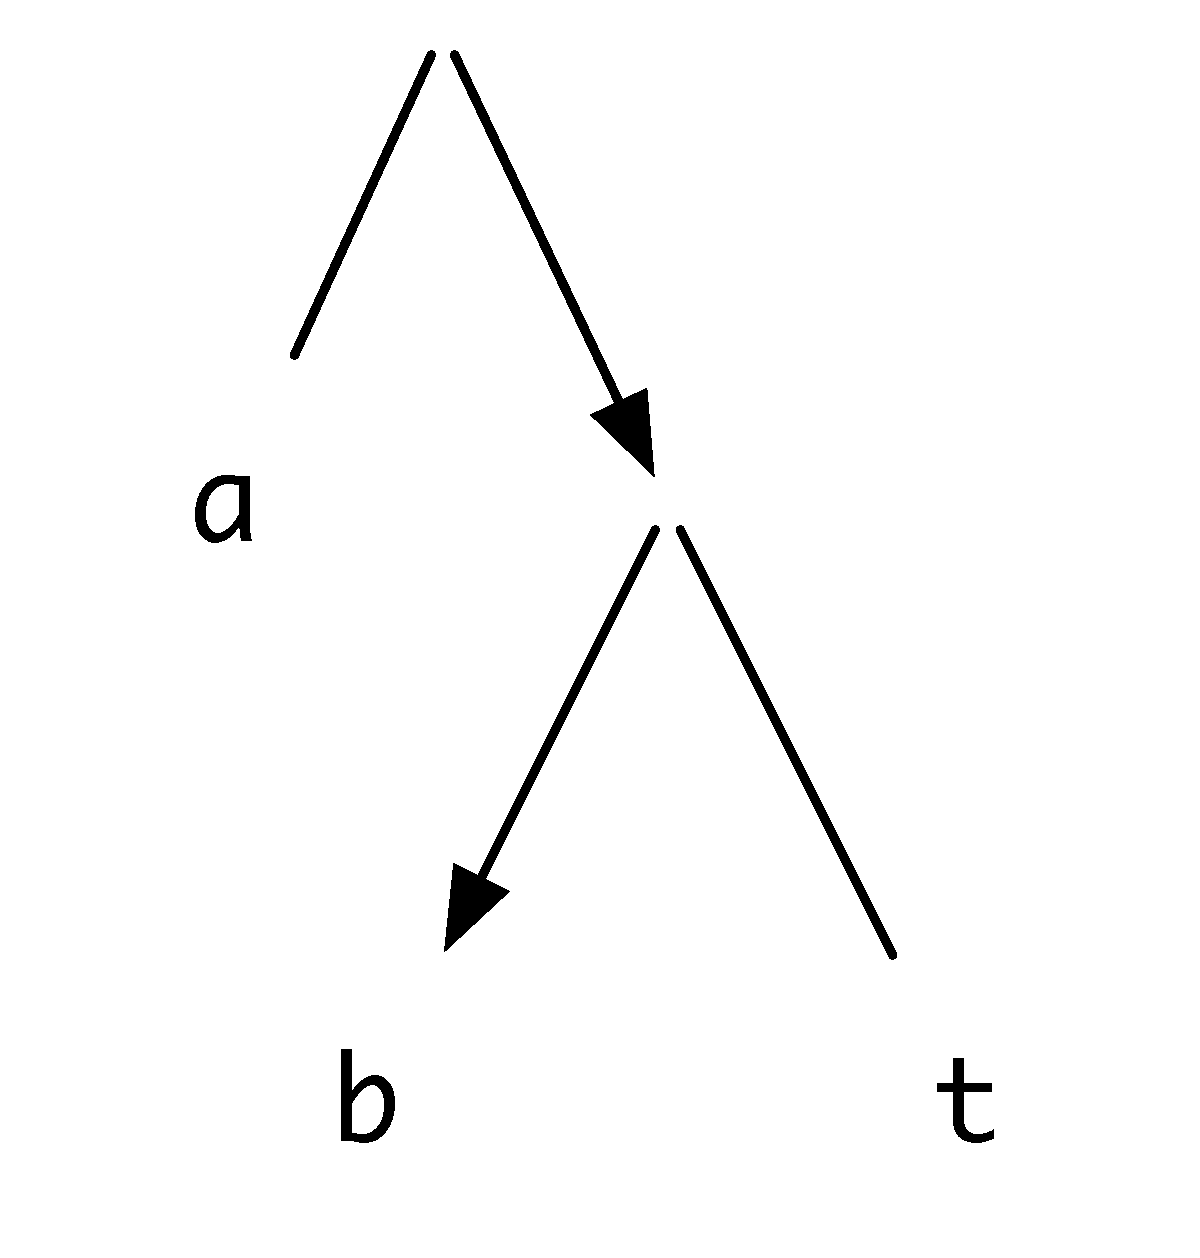
\includegraphics[width=1in]{Pictures/Huffman2.pdf}
\end{center}
which gives \texttt{b} the code \texttt{RL}. Similarly, \texttt{L} codes \texttt{a}, and
\texttt{RR} the letter \texttt{t}. 

The codes given by trees are  \textbf{prefix codes}\index{coding!prefix codes}; in these codes 
no code for a letter is the start (or prefix) of the code for another. This is
because no route to a leaf of the tree can be the start of the route to
another leaf. For more information about Huffman codes and
a wealth of general material on algorithms, see \citeN{cormen}.

A message is also \textbf{decoded} using the tree. Consider the message
\texttt{RLLRRRRLRR}. To decode we follow the route through the tree given,
moving right then left, to give the letter \texttt{b},
\begin{center}
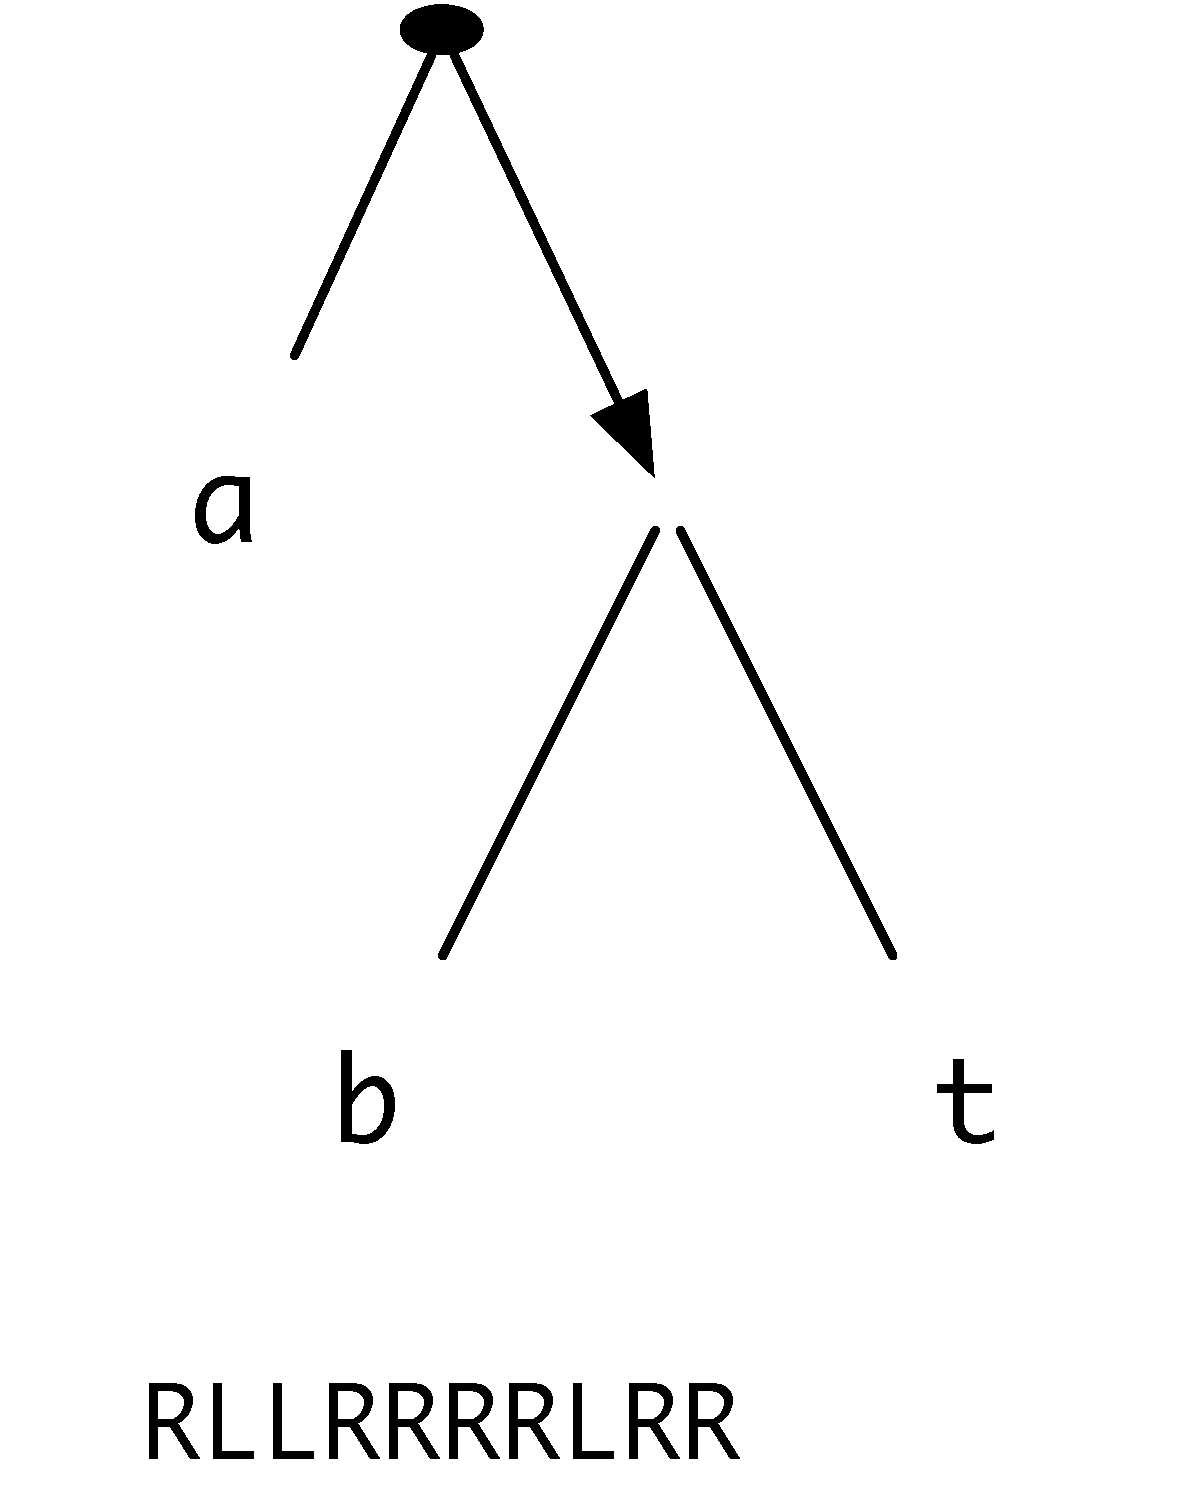
\includegraphics[width=1in]{Pictures/Huffman3.pdf}\hfill
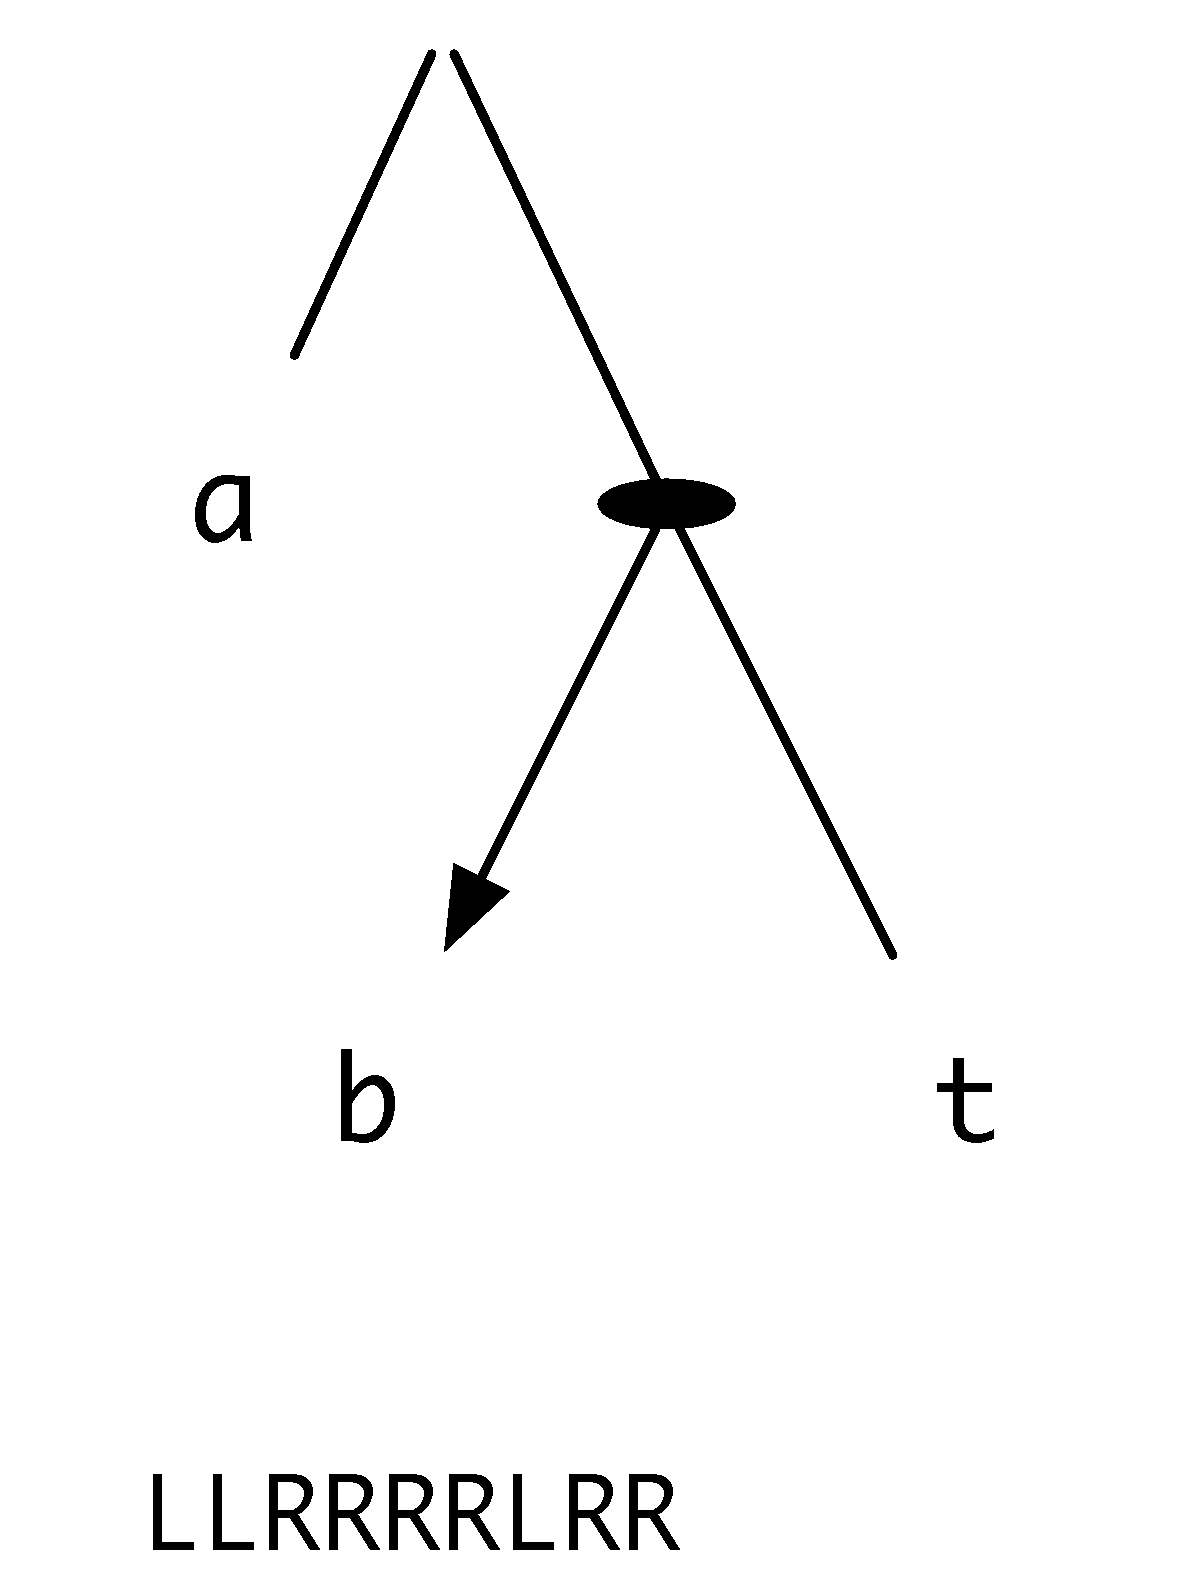
\includegraphics[width=1in]{Pictures/Huffman4.pdf}\hfill
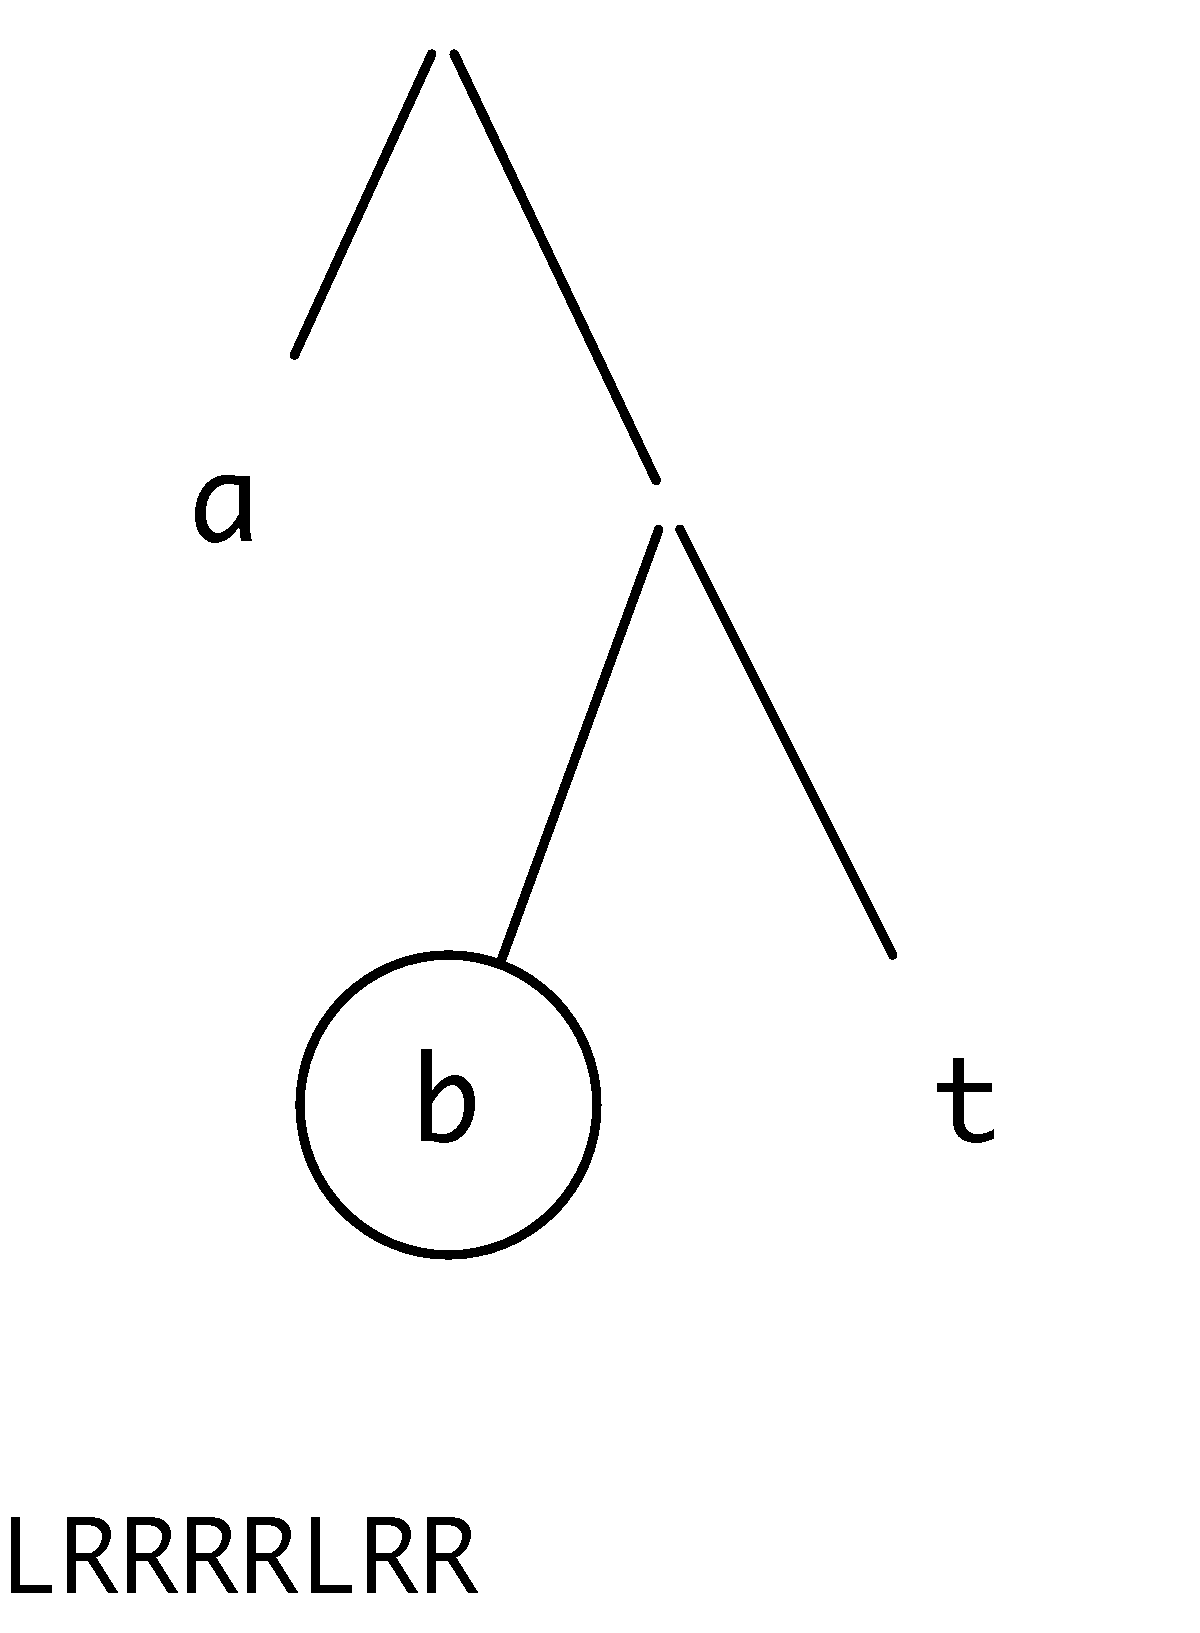
\includegraphics[width=1in]{Pictures/Huffman5.pdf}
\end{center}
where we have shown under each tree the sequence of bits remaining to be
decoded. Continuing again from the top, we have the codes for \texttt{a} then
\texttt{t},  
\begin{center}
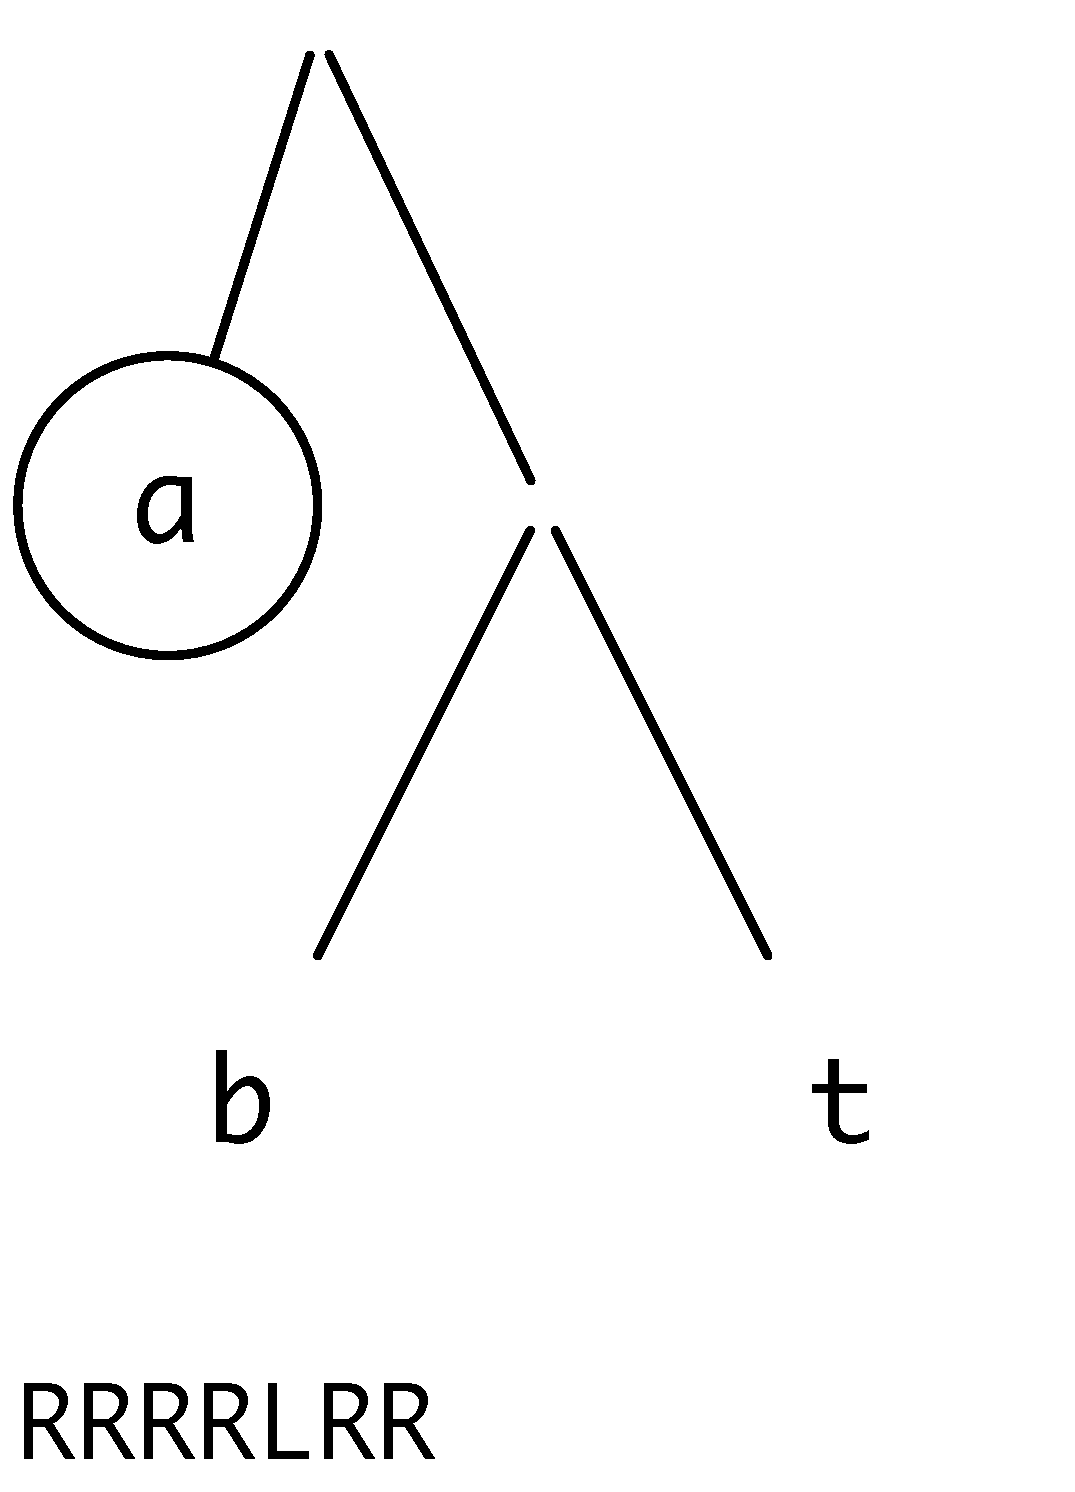
\includegraphics[width=1in]{Pictures/Huffman6.pdf}\hfill
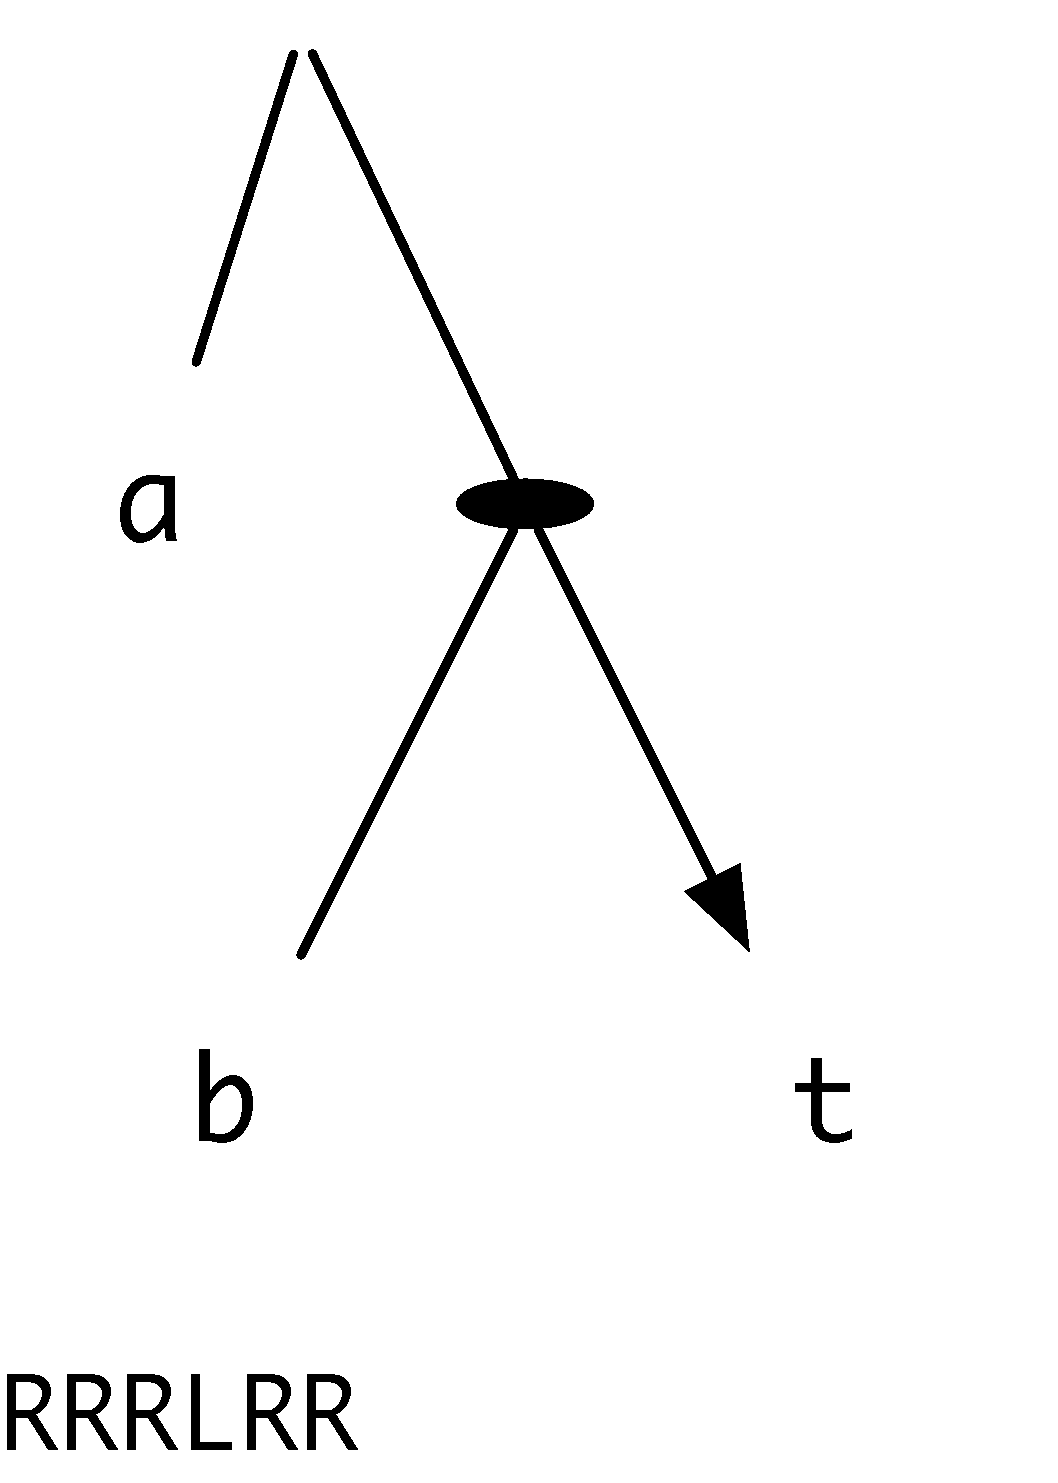
\includegraphics[width=1in]{Pictures/Huffman7.pdf}\hfill
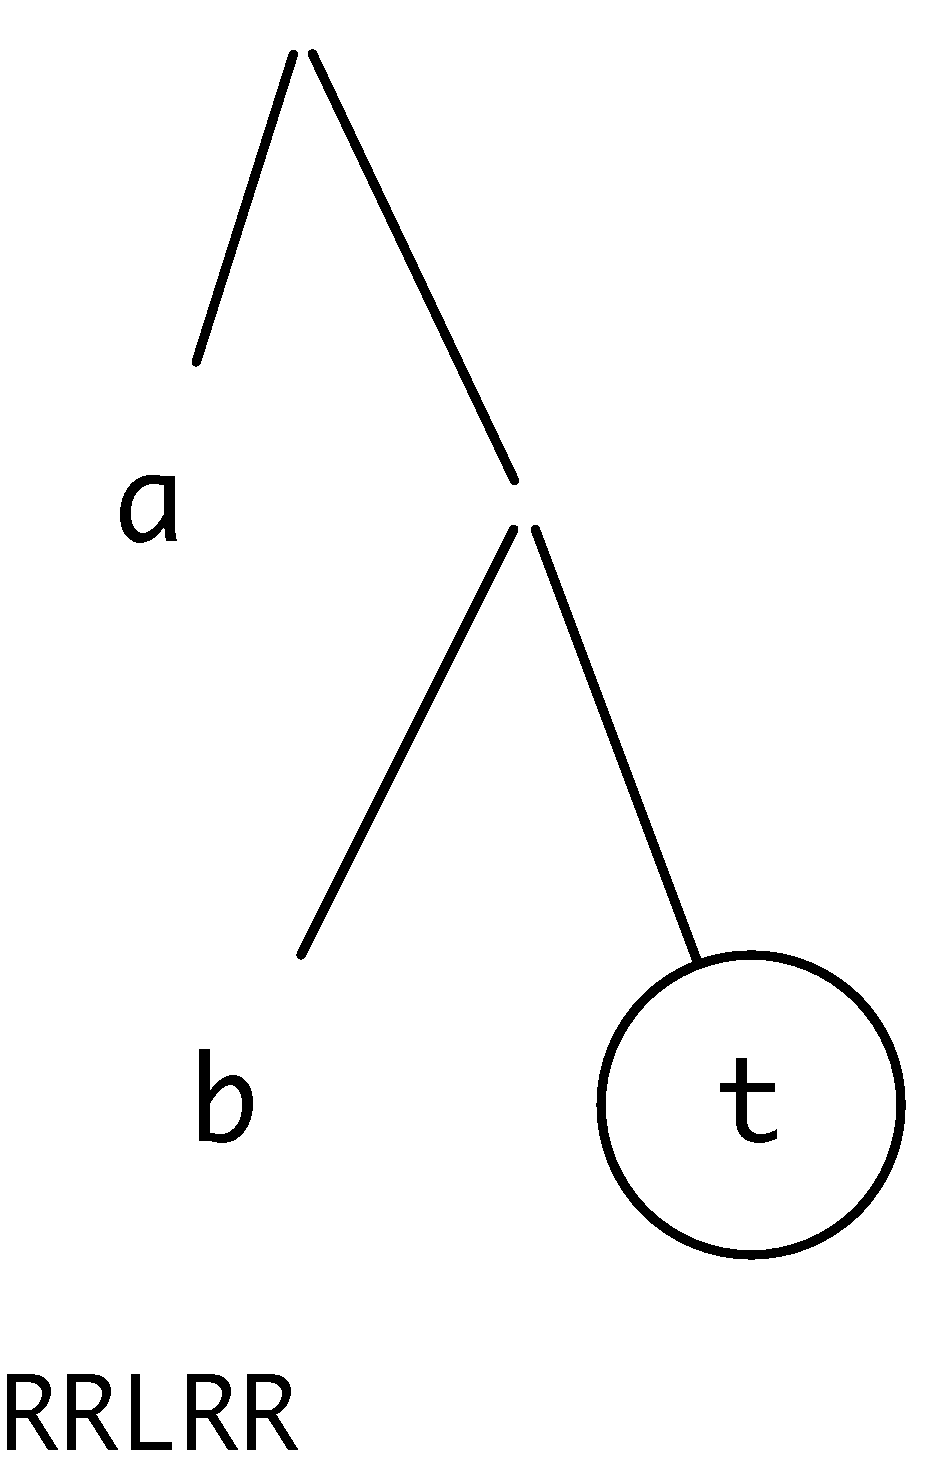
\includegraphics[width=0.9in]{Pictures/Huffman8.pdf}
\end{center}
so
the decoded message begins with the letters \texttt{bat}. 

In full, the message is \texttt{battat}, and the coded message is ten bits
long. The codes for individual characters are of different lengths; \texttt{a}
is coded in one bit, and the other characters in two. Is this a wise choice of
code in view of a message in which the letter \texttt{t} predominates? Using the
tree
\begin{center}
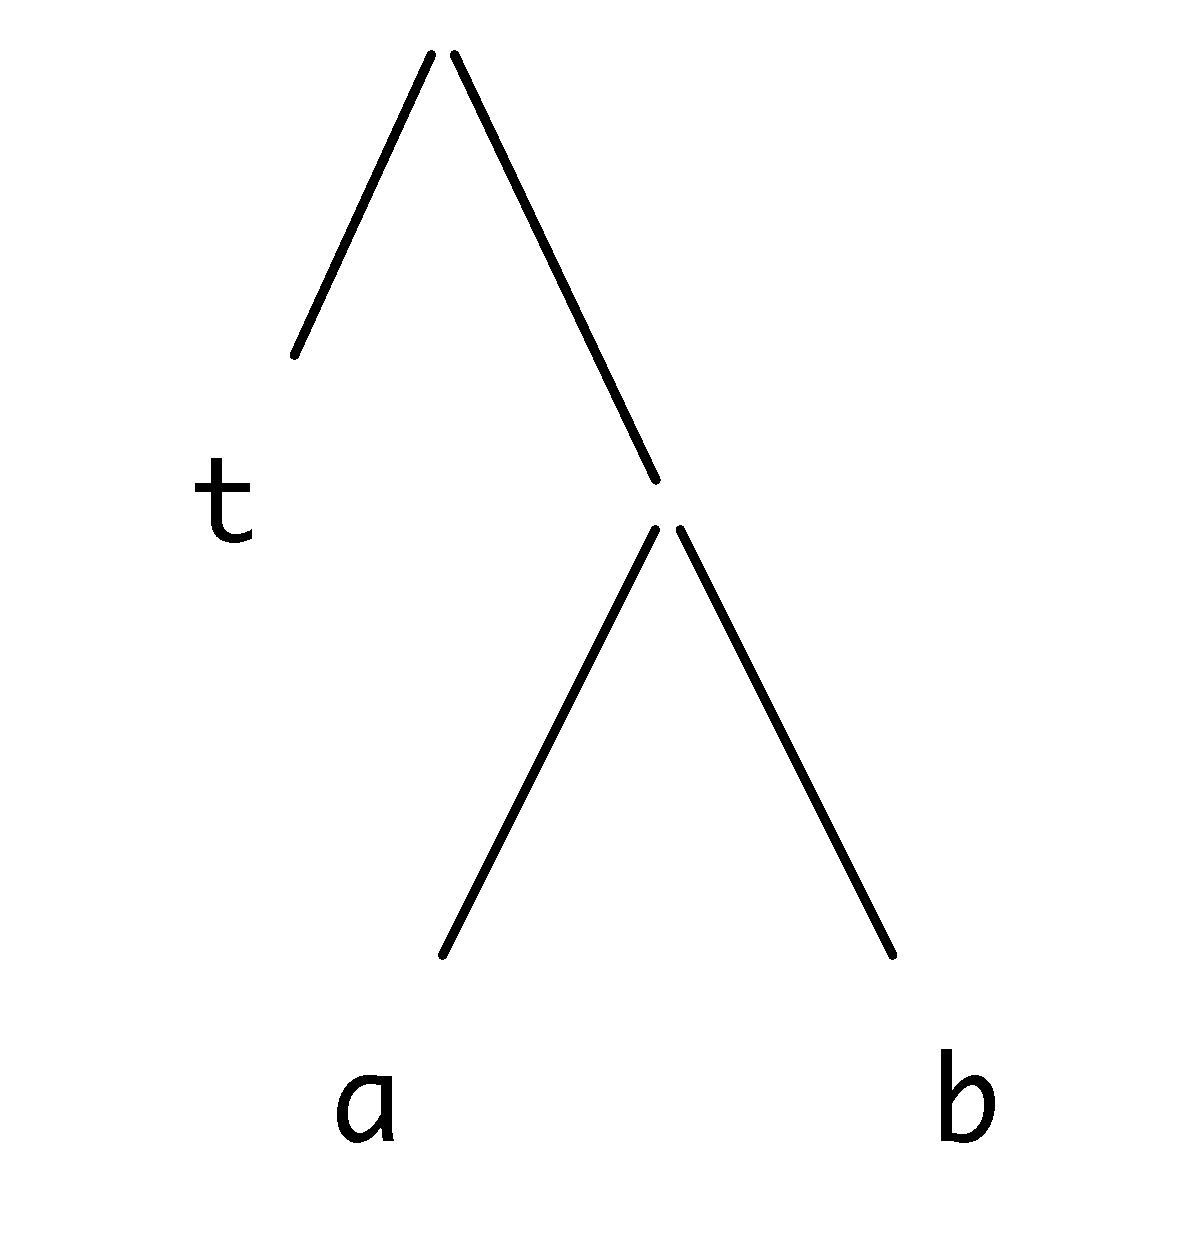
\includegraphics[width=1in]{Pictures/Huffman9.pdf}
\end{center}
the coded message becomes \texttt{RRRLLLRLL}, a nine-bit coding. A
Huffman\index{coding!Huffman} code is built so that the most frequent letters have the shortest
sequences of code bits, and the less frequent have more `expensive' code
sequences, justified by the rarity of their occurrence; Morse code is an
example of a Huffman code in common use.

The remainder of the chapter explores the implementation of Huffman coding,
illustrating the module system of Haskell.
\index{coding|)}

\begin{exercises}

\item
What is the coding of the message \texttt{battat} using the following
tree?
\begin{center}
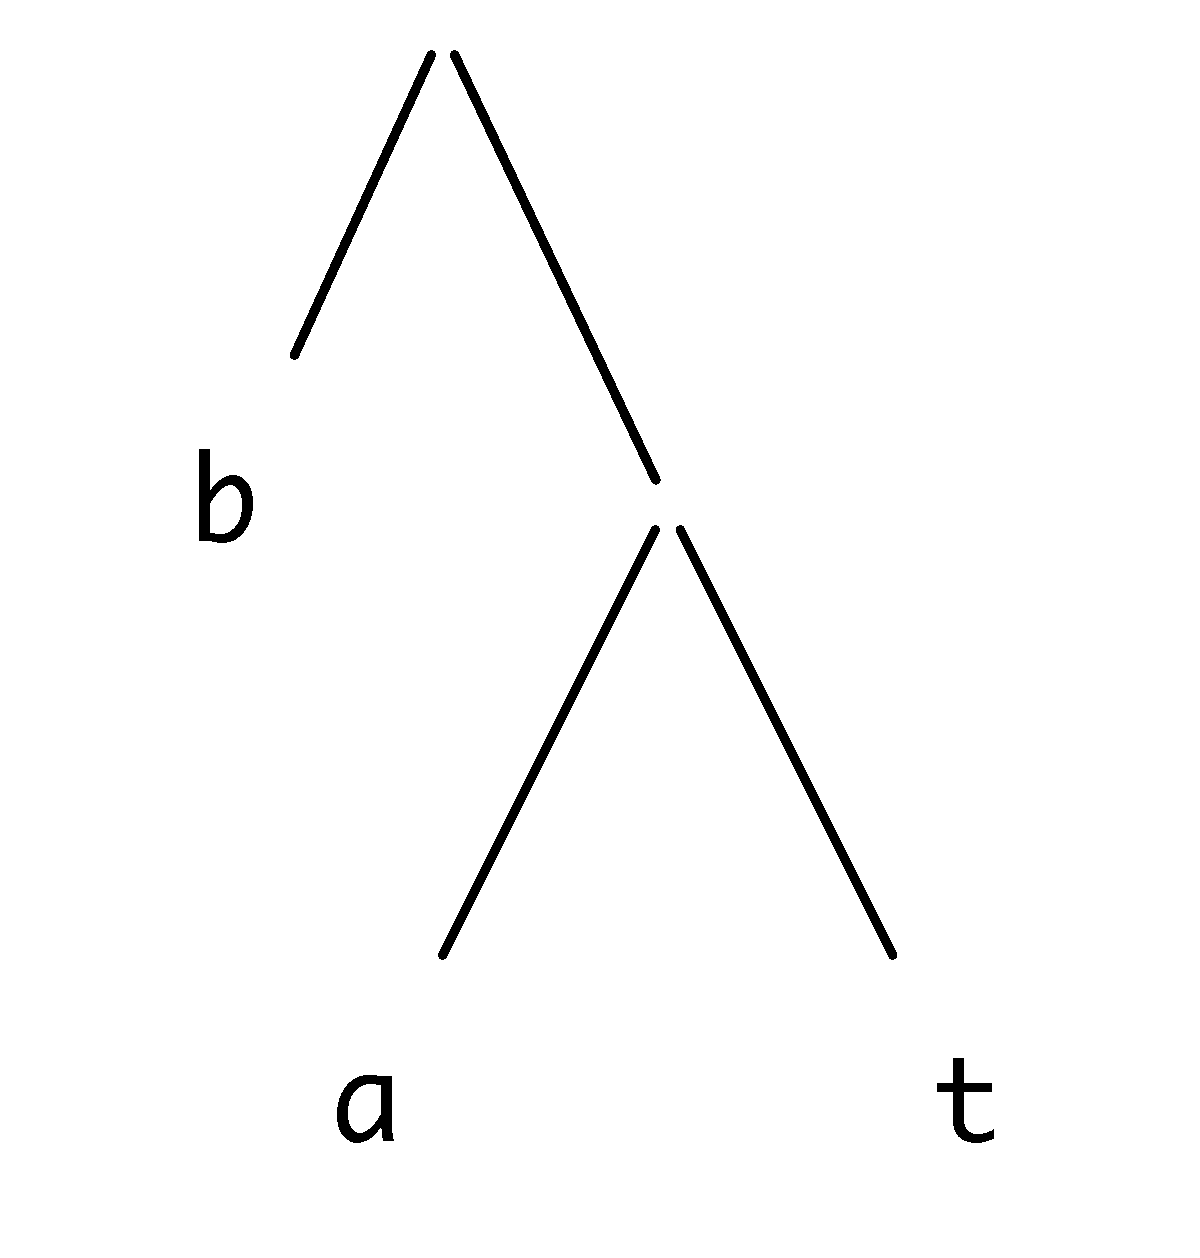
\includegraphics[width=1in]{Pictures/Huffman10.pdf}
\end{center}
Compare the length of the coding with the others given earlier. 

\item
Using the first coding tree, decode the coded
message \texttt{RLLRLRLLRR}. Which tree
would you expect to give the best coding of the message? Check your answer by
trying the three possibilities.
\end{exercises}


\section{Implementation -- I}

We now begin to implement the Huffman coding and decoding, in a series of
Haskell modules. The overall structure of the system we develop is illustrated
at the end of the chapter in Figure \ref{overallMod}. 

As earlier, we first develop the
types used in the system.

\subsection*{The types -- \texttt{Types.hs}}
\minx{Types.hs}

The codes are sequences of bits, so we define
\begin{alltt}
data Bit   =  L | R deriving (Eq,Show)\minx{Bit}\minx{HCode}
type HCode = [Bit]
\end{alltt}
and in the translation we will convert the Huffman tree to a table for ease
of coding.
\begin{alltt}
type Table = [ (Char,HCode) ]\minx{Table}
\end{alltt}
The Huffman trees themselves carry characters at the leaves. We shall see
presently that during their formation we also use information about the
frequency with which each character appears; hence the inclusion of 
integers
both at the leaves and at the internal nodes.
\begin{alltt}
data Tree = Leaf Char Int |\minx{Tree}
            Node Int Tree Tree
\end{alltt}
The file containing the module is illustrated in Figure
\ref{typeMod}.
\begin{figure}
\begin{alltt}
--         Types.hs							
--  
--         The types used in the Huffman coding example.			

-- The interface to the module Types is written out		
-- explicitly here, after the module name.                    	

module Types ( Tree(Leaf,Node), 
               Bit(L,R),  
               HCode , 
               Table  ) where

-- Trees to represent the relative frequencies of characters 	
-- and therefore the Huffman codes.						

data Tree = Leaf Char Int | Node Int Tree Tree

-- The types of bits, Huffman codes and tables of Huffman codes.	

data Bit = L | R deriving (Eq,Show)

type HCode = [Bit]

type Table = [ (Char,HCode) ]
\end{alltt}
\caption{The file \texttt{Types.hs}.}
\label{typeMod}
\end{figure}
The name of the file, with an indication of its purpose, is listed at the 
start of the file; each of the definitions is preceded by a comment as to its
purpose.

Note that we have given a full description of what is exported by the module,
by listing the items after the module name. For the \texttt{data} types which
are exported, \texttt{Tree} and 
\texttt{Bit}, the
constructors are exported explicitly; this could also be done by following their names
with \texttt{(..)}. 
This interface information could have been omitted, but we include it here as useful
documentation of the interface to the module.
\index{modules!interface documentation}

\subsection*{Coding and decoding -- \texttt{Coding.hs}}
\minx{Coding.hs}

This module uses the types in \texttt{Types.hs}, and so imports them like this
\begin{alltt}
\mbox{import Types ( Tree(Leaf,Node), Bit(L,R), HCode, Table )}
\end{alltt}
We have chosen to list the names imported here; the statement \texttt{import
Types} would have the same effect, but would lose the extra documentation.

The purpose of the module is to define functions to code and decode
messages: we export only these, and not the auxiliary function(s) which may
be used in their definition. Our module therefore has the header
\begin{alltt}
module Coding ( codeMessage , decodeMessage ) 
\end{alltt}
To code a message according to a table of
codes, we look up each character in the table, and concatenate the results.
\begin{alltt}
codeMessage :: Table -> [Char] -> HCode\minx{codeMessage}

codeMessage tbl = concat . map (lookupTable tbl)
\end{alltt}
It is interesting to see that the function level definition here gives an
exact implementation of the description which precedes it; using partial
application and function composition has made the definition clearer.

We now define \texttt{lookupTable}, which is a standard
function to look up the value corresponding to a `key' in a table.
\begin{alltt}
lookupTable :: Table -> Char -> HCode\minx{lookupTable}

lookupTable [] c = error "lookupTable"
lookupTable ((ch,n):tb) c
  | ch==c       = n
  | otherwise   = lookupTable tb c 
\end{alltt}
Because it is not included in the list of identifiers in the  \texttt{module} statement above, this definition is not exported.

To decode a message, which is a sequence of bits,  that is an element of
\texttt{HCode}, we use a \texttt{Tree}. 
\begin{alltt}
decodeMessage :: Tree -> HCode -> [Char]\minx{decodeMessage}
\end{alltt}
We saw in Section \ref{codeIntro} that decoding according to the tree \texttt{tr}
has two main cases. 
\begin{titemize}
\item If we are at an internal \texttt{Node}, we choose the sub-tree dictated by
the first bit of the code.
\item If at a leaf, we read off the character found, and then begin to decode
the remainder of the code at the top of the tree \texttt{tr}.
\end{titemize}
When the code is exhausted, so is the decoded message.
\begin{alltt}
decodeMessage tr
  = decodeByt tr
    where
    decodeByt (Node n t1 t2) (L:rest)
      = decodeByt t1 rest
    decodeByt (Node n t1 t2) (R:rest)
      = decodeByt t2 rest
    decodeByt (Leaf c n) rest
      = c : decodeByt tr rest
    decodeByt t [] = []
\end{alltt}
The locally defined function is called \texttt{decodeByt} because it decodes `by
\texttt{t}'.

The first coding tree and example message of Section \ref{codeIntro} can be
given by
\begin{alltt}
exam1 = Node 0 (Leaf 'a' 0)
               (Node 0 (Leaf 'b' 0) (Leaf 't' 0))
mess1 = [R,L,L,R,R,R,R,L,R,R]
\end{alltt}
and decoding of this message begins thus
\begin{alltt}
decodeMessage exam1 mess1
\step decodeByt exam1 mess1
\step decodeByt exam1 [R,L,L,R,R,R,R,L,R,R]
\step decodeByt (Node 0 (Leaf 'b' 0) (Leaf 't' 0)) 
                                 [L,L,R,R,R,R,L,R,R]
\step decodeByt (Leaf 'b' 0) [L,R,R,R,R,L,R,R]
\step 'b' : decodeByt exam1 [L,R,R,R,R,L,R,R] 
\step 'b' : decodeByt (Leaf 'a' 0) [R,R,R,R,L,R,R]
\step 'b' : 'a' : decodeByt exam1 [R,R,R,R,L,R,R] 
\end{alltt}
Before looking at the implementation any further, we look at how to construct
the Huffman coding tree, given a text.

\begin{exercises}

\item
Complete the calculation of \texttt{decodeMessage exam1 mess1} begun above.

\item
With the table
\begin{alltt}
table1 = [ ('a',[L]) , ('b',[R,L]) , ('t',[R,R]) ]
\end{alltt}
give a calculation of 
\begin{alltt}
codeMessage table1 "battab"
\end{alltt}
\end{exercises}
\section{Building Huffman trees}
%\index{Huffman trees!building}

Given a text, such as \texttt{"battat"}, how do we find the tree giving the
optimal code for the text? We explain it in a number of
stages following Section 17.3
of \citeN{cormen}.
\begin{titemize} 
\item We first find the frequencies of the
individual letters, in this case giving
\begin{alltt}
[('b',1),('a',2),('t',3)]
\end{alltt}
\item The main idea of the translation is to build the tree by taking the two
characters occurring least frequently, and making a {\em single\/} character
(or {\em tree\/}) of them. This process is repeated until a single tree
results; the steps which follow give this process in more detail.
\item Each of \texttt{('b',1)}, \ldots\ is turned into a tree, giving the list of
trees
\begin{alltt}
[ Leaf 'b' 1 , Leaf 'a' 2 , Leaf 't' 3 ]
\end{alltt}
which is sorted into frequency order.
\item We then begin to {\em amalgamate together\/} trees: we take the two
trees of lowest frequency, put them together, and insert the result in the
appropriate place to preserve the frequency order.
\begin{alltt}
[ Node 3 (Leaf 'b' 1) (Leaf 'a' 2) , Leaf 't' 3 ]
\end{alltt}
\item This process is repeated, until a single tree results
\begin{alltt}
Node 6 (Node 3 (Leaf 'b' 1) (Leaf 'a' 2)) (Leaf 't' 3)
\end{alltt}
which is pictured like this
\begin{center}
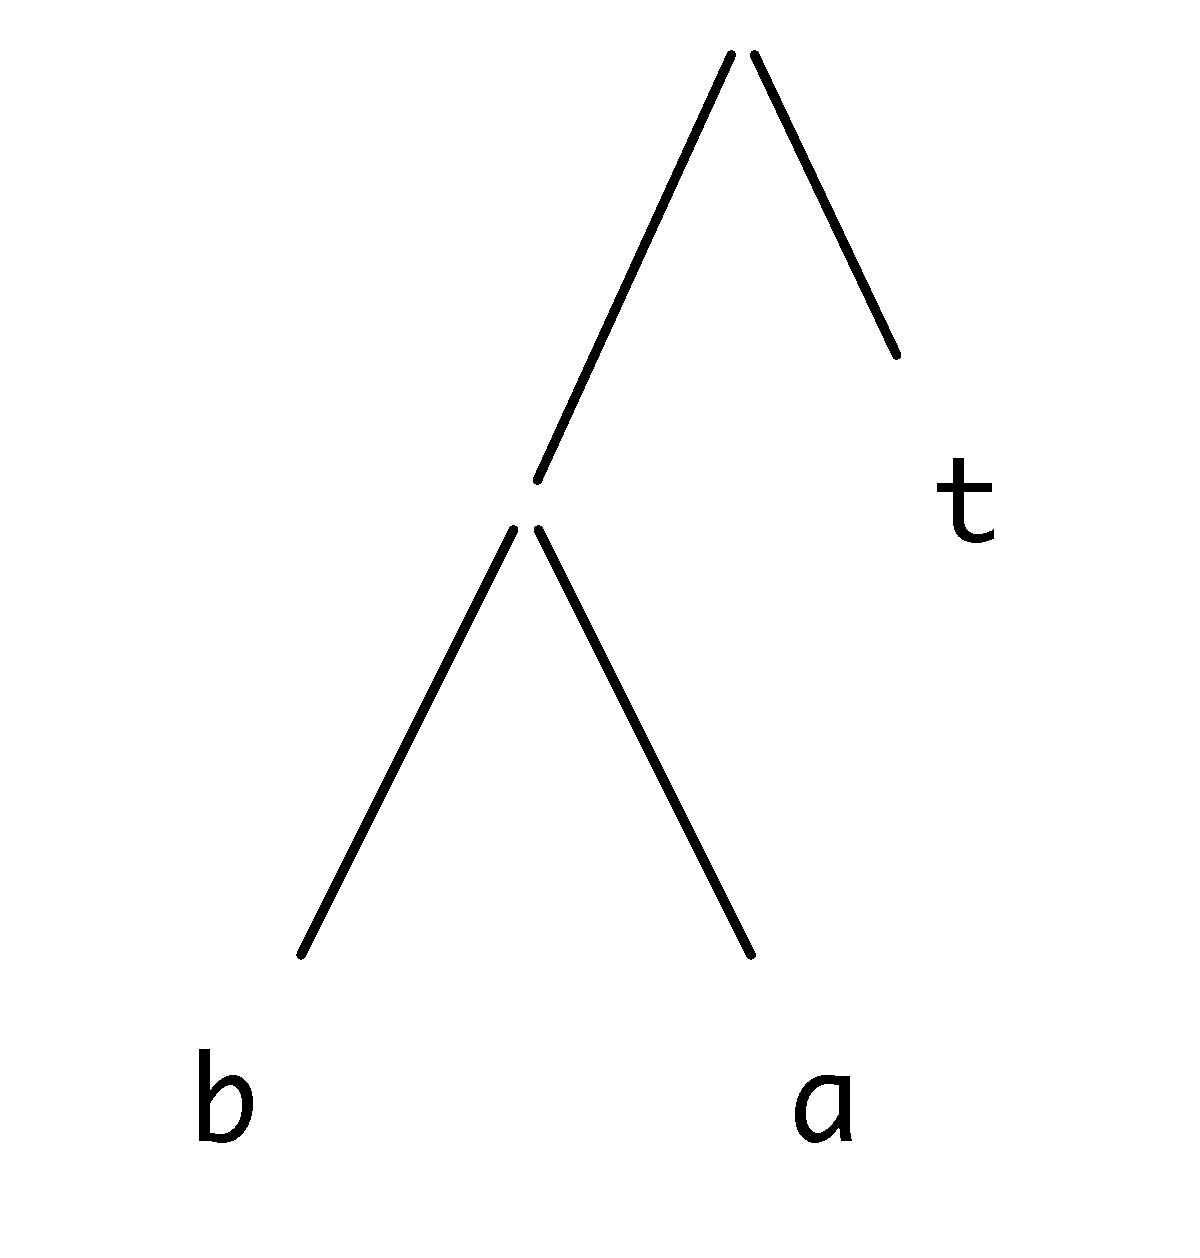
\includegraphics[width=1in]{Pictures/Huffman11.pdf}
\end{center}
\item This tree can then be turned into a \texttt{Table}
\begin{alltt}
[ ('b',[L,L]) , ('a',[L,R]) , ('t',[R]) ]
\end{alltt}
\end{titemize}
We now look at how the system is implemented in Haskell.

\section{Design}
\index{design!Huffman coding system}

Implementing the system will involve us in designing various modules to
perform the stages given above. We start by deciding what the modules will
be  and the functions that they will implement. This is the equivalent at the
larger scale of \textbf{divide and conquer}\index{divide and conquer};
we separate the problem into
manageable portions, which can be solved separately, and which are put
together using the \texttt{import} and \texttt{module} statements. We design
these \textbf{interfaces} \index{interface}before implementing the functions.

The three stages of conversion are summarized in Figure \ref{codeDesign},
which shows the module directives of the three component files. We have added
as comments the types of objects to be exported, so that these directives
contain enough information for the exported functions in the
files to be used without knowing {\em how\/} they are defined. 

\begin{figure}\begin{alltt}
Frequency.hs:

module Frequency ( frequency )  -- [Char] -> [(Char,Int)]

\hrulefill

MakeTree.hs:

module MakeTree ( makeTree )    -- [(Char,Int)] -> Tree
import Types

\hrulefill

CodeTable.hs:

module CodeTable ( codeTable )  -- Tree -> Table
import Types 
\end{alltt}
\caption{Module directives for Huffman tree formation.}
\label{codeDesign}
\end{figure}
In fact the component functions \texttt{frequency} and \texttt{makeTree} will
never be used separately, and so we compose them in the module 
\texttt{MakeCode.hs} when bringing the three files together. This is given in Figure
\ref{makeCode}.

\begin{figure}
\begin{alltt}
-- 								
--         MakeCode.hs							
-- 								
--         Huffman coding in Haskell.					
-- 								

module MakeCode ( codes, codeTable ) where

import Types
import Frequency ( frequency )
import MakeTree  ( makeTree )
import CodeTable ( codeTable )

-- Putting together frequency calculation and tree conversion	

codes :: [Char] -> Tree

codes = makeTree . frequency
\end{alltt}
\caption{The module \texttt{MakeCode.hs}.}
\label{makeCode}
\end{figure}
Our next task is to implement each module in full and we turn to that now.

\section{Implementation -- II}

In this section we discuss in turn the three implementation modules.

\subsection*{Counting characters --- \texttt{Frequency.hs}}
\minx{Frequency.hs}

The aim of the function \texttt{frequency}\minx{frequency} is to take a text such as 
\texttt{"battat"} to a list of characters, in increasing frequency of occurrence,
\texttt{[('b',1),('a',2),('t',3)]}. We do this in three stages:
\begin{titemize}
\item First we pair each character with the count of \texttt{1}, giving
\begin{alltt}
[('b',1),('a',1),('t',1),('t',1),('a',1),('t',1)]
\end{alltt}
\item Next, we sort the list on the characters, bringing together the counts of
equal characters.
\begin{alltt}
[('a',2),('b',1),('t',3)]
\end{alltt}
\item Finally, we sort the list into increasing frequency order, to give the
list above.
\end{titemize}
The function uses two different sorts -- one on character, one on
frequency -- to achieve its result. Is there any way we can define a single
sorting function to perform both sorts? 

We can give a general merge sort
\index{sorting!merge sort}
function, which works by \textbf{merging}, in order, the results of sorting the
front and rear halves of the list.
\begin{alltt}
mergeSort :: ([a]->[a]->[a]) -> [a] -> [a]\minx{mergeSort}

mergeSort merge xs
  | length xs < 2 	= xs					
  | otherwise		
      = merge (mergeSort merge first)
              (mergeSort merge second)	
        where
        first  = take half xs
        second = drop half xs
        half   = (length xs) `div` 2
\end{alltt}
The first argument to \texttt{mergeSort} is the merging function, which takes
two sorted lists and merges their contents in order. It is by making this
operation a {\em parameter\/} that the \texttt{mergeSort} function becomes
reusable.

In sorting the characters, we amalgamate entries for the same character
\begin{alltt}\minx{alphaMerge}
alphaMerge :: [(Char,Int)] -> [(Char,Int)] -> [(Char,Int)]	

alphaMerge xs [] = xs
alphaMerge [] ys = ys
alphaMerge ((p,n):xs) ((q,m):ys)
  | (p==q)      = (p,n+m) : alphaMerge xs ys		
  | (p<q)       = (p,n) : alphaMerge xs ((q,m):ys)	
  | otherwise   = (q,m) : alphaMerge ((p,n):xs) ys	
\end{alltt}
while when sorting on frequency we compare frequencies; when two
pairs have the same frequency, we order according to the character ordering.
\begin{alltt}\minx{freqMerge}
freqMerge :: [(Char,Int)] -> [(Char,Int)] -> [(Char,Int)]	

freqMerge xs [] = xs
freqMerge [] ys = ys
freqMerge ((p,n):xs) ((q,m):ys)
  | (n<m || (n==m && p<q)) 
    = (p,n) : freqMerge xs ((q,m):ys)	
  | otherwise 
    = (q,m) : freqMerge ((p,n):xs) ys	
\end{alltt}
We can now give the top-level definition of \texttt{frequency}
\begin{alltt}
frequency :: [Char] -> [ (Char,Int) ]\minx{frequency}

frequency
  = mergeSort freqMerge . mergeSort alphaMerge . map start
    where
    start ch = (ch,1)
\end{alltt}
which we can see is a direct combination of the three stages listed in the
informal description of the algorithm.

Note that of all the functions defined in this module, only \texttt{frequency}
is exported.

\subsection*{Making the Huffman tree -- \texttt{MakeTree.hs}}
\minx{MakeTree.hs}

We have two stages in making a Huffman tree from a list of characters with
their frequencies.
\begin{alltt}
makeTree :: [ (Char,Int) ] -> Tree\minx{makeTree}
makeTree  = makeCodes . toTreeList
\end{alltt}
where
\begin{alltt}\minx{toTreeList}\minx{makeCodes}
toTreeList :: [ (Char,Int) ] -> [Tree]
makeCodes  :: [Tree] -> Tree
\end{alltt}
The function \texttt{toTreeList} converts each character-number pair into a
tree, thus
\begin{alltt}
toTreeList = map (uncurry Leaf)
\end{alltt}
where note that we use the prelude function \texttt{uncurry} to make an uncurried version
of the constructor function \texttt{Leaf}.

The function \texttt{makeCodes} amalgamates trees successively into a single
tree
\begin{alltt}
makeCodes [t] = t
makeCodes ts  = makeCodes (amalgamate ts)
\end{alltt}
How are trees amalgamated? We have to pair together the first two trees in
the list (since the list is kept in ascending order of frequency) and then
insert the result in the list preserving the frequency order. Working top-down, we have 
\begin{alltt}
amalgamate :: [ Tree ] -> [ Tree ]

amalgamate (t1:t2:ts) = insTree (pair t1 t2) ts
\end{alltt}
When we pair two trees, we need to combine their frequency counts, so
\begin{alltt}
pair :: Tree -> Tree -> Tree

pair t1 t2 = Node (v1+v2) t1 t2
             where
             v1 = value t1
             v2 = value t2
\end{alltt}
where the value of a tree is given by
\begin{alltt}
value :: Tree -> Int

value (Leaf _ n)   = n
value (Node n _ _) = n
\end{alltt}
The definition of \texttt{insTree}, which is similar to that used in an insertion
sort, is left as an exercise. Again, the definition of the exported function
uses various others whose definitions are not visible to the `outside world'.

\subsection*{The code table -- \texttt{CodeTable.hs}}
\minx{CodeTable.hs}

Here we give the function \texttt{codeTable} which takes a Huffman tree into a
code table. In converting the tree \texttt{Node n t1 t2} we have to convert 
\texttt{t1}, adding \texttt{L} at the front of the code, and \texttt{t2} with \texttt{R} at
the head. We therefore write the more general conversion function
\begin{alltt}
convert :: HCode -> Tree -> Table\minx{convert}
\end{alltt}
whose first argument is the `path so far' into the tree. The definition is
\begin{alltt}
convert cd (Leaf c n) 
      =  [(c,cd)]
convert cd (Node n t1 t2)
      = (convert (cd++[L]) t1) ++ (convert (cd++[R]) t2)
\end{alltt}
The \texttt{codeTable} function is given by starting the conversion with an
empty code string
\begin{alltt}\minx{codeTable}
codeTable :: Tree -> Table
codeTable = convert []
\end{alltt}
Consider the calculation of
\begin{alltt}
codeTable (Node 6 (Node 3 (Leaf 'b' 1) (Leaf 'a' 2)) 
                  (Leaf 't' 3))
\step convert [] (Node 6 (Node 3 (Leaf 'b' 1) (Leaf 'a' 2)) 
                       (Leaf 't' 3))
\step convert [L] (Node 3 (Leaf 'b' 1) (Leaf 'a' 2)) ++
    convert [R] (Leaf 't' 3)
\step convert [L,L] (Leaf 'b' 1) ++ 
    convert [L,R] (Leaf 'a' 2) ++ 
    [ ('t',[R]) ]
\step [ ('b',[L,L]) , ('a',[L,R]) , ('t',[R]) ]
\end{alltt}

\begin{figure}[t]
\begin{center}
\begin{alltt}
-- The main module of the Huffman example

module Main (main, codeMessage, decodeMessage, codes, codeTable ) where

import Types    ( Tree(Leaf,Node), Bit(L,R), HCode , Table )
import Coding   ( codeMessage, decodeMessage ) 
import MakeCode ( codes, codeTable )

-- Main expression: print the coded and decoded 
-- example text "there is a green hill".
main = print decoded

-- The example message to be coded.
message :: String
message = "there are green hills here"

-- The Huffman tree generated from the example.
treeEx :: Tree
treeEx = codes "there is a green hill"

-- The coding table generated from the example.					
tableEx :: Table
tableEx = codeTable (codes "there is a green hill")

-- The example in code.
coded :: HCode
coded = codeMessage tableEx message

-- The example coded and then decoded.
decoded :: String
decoded = decodeMessage treeEx coded
\end{alltt}
\end{center}
\caption{The \texttt{Main} module of the Huffman coding system.}
\label{mainMod}
\end{figure}


\begin{figure}[t]
\begin{center}
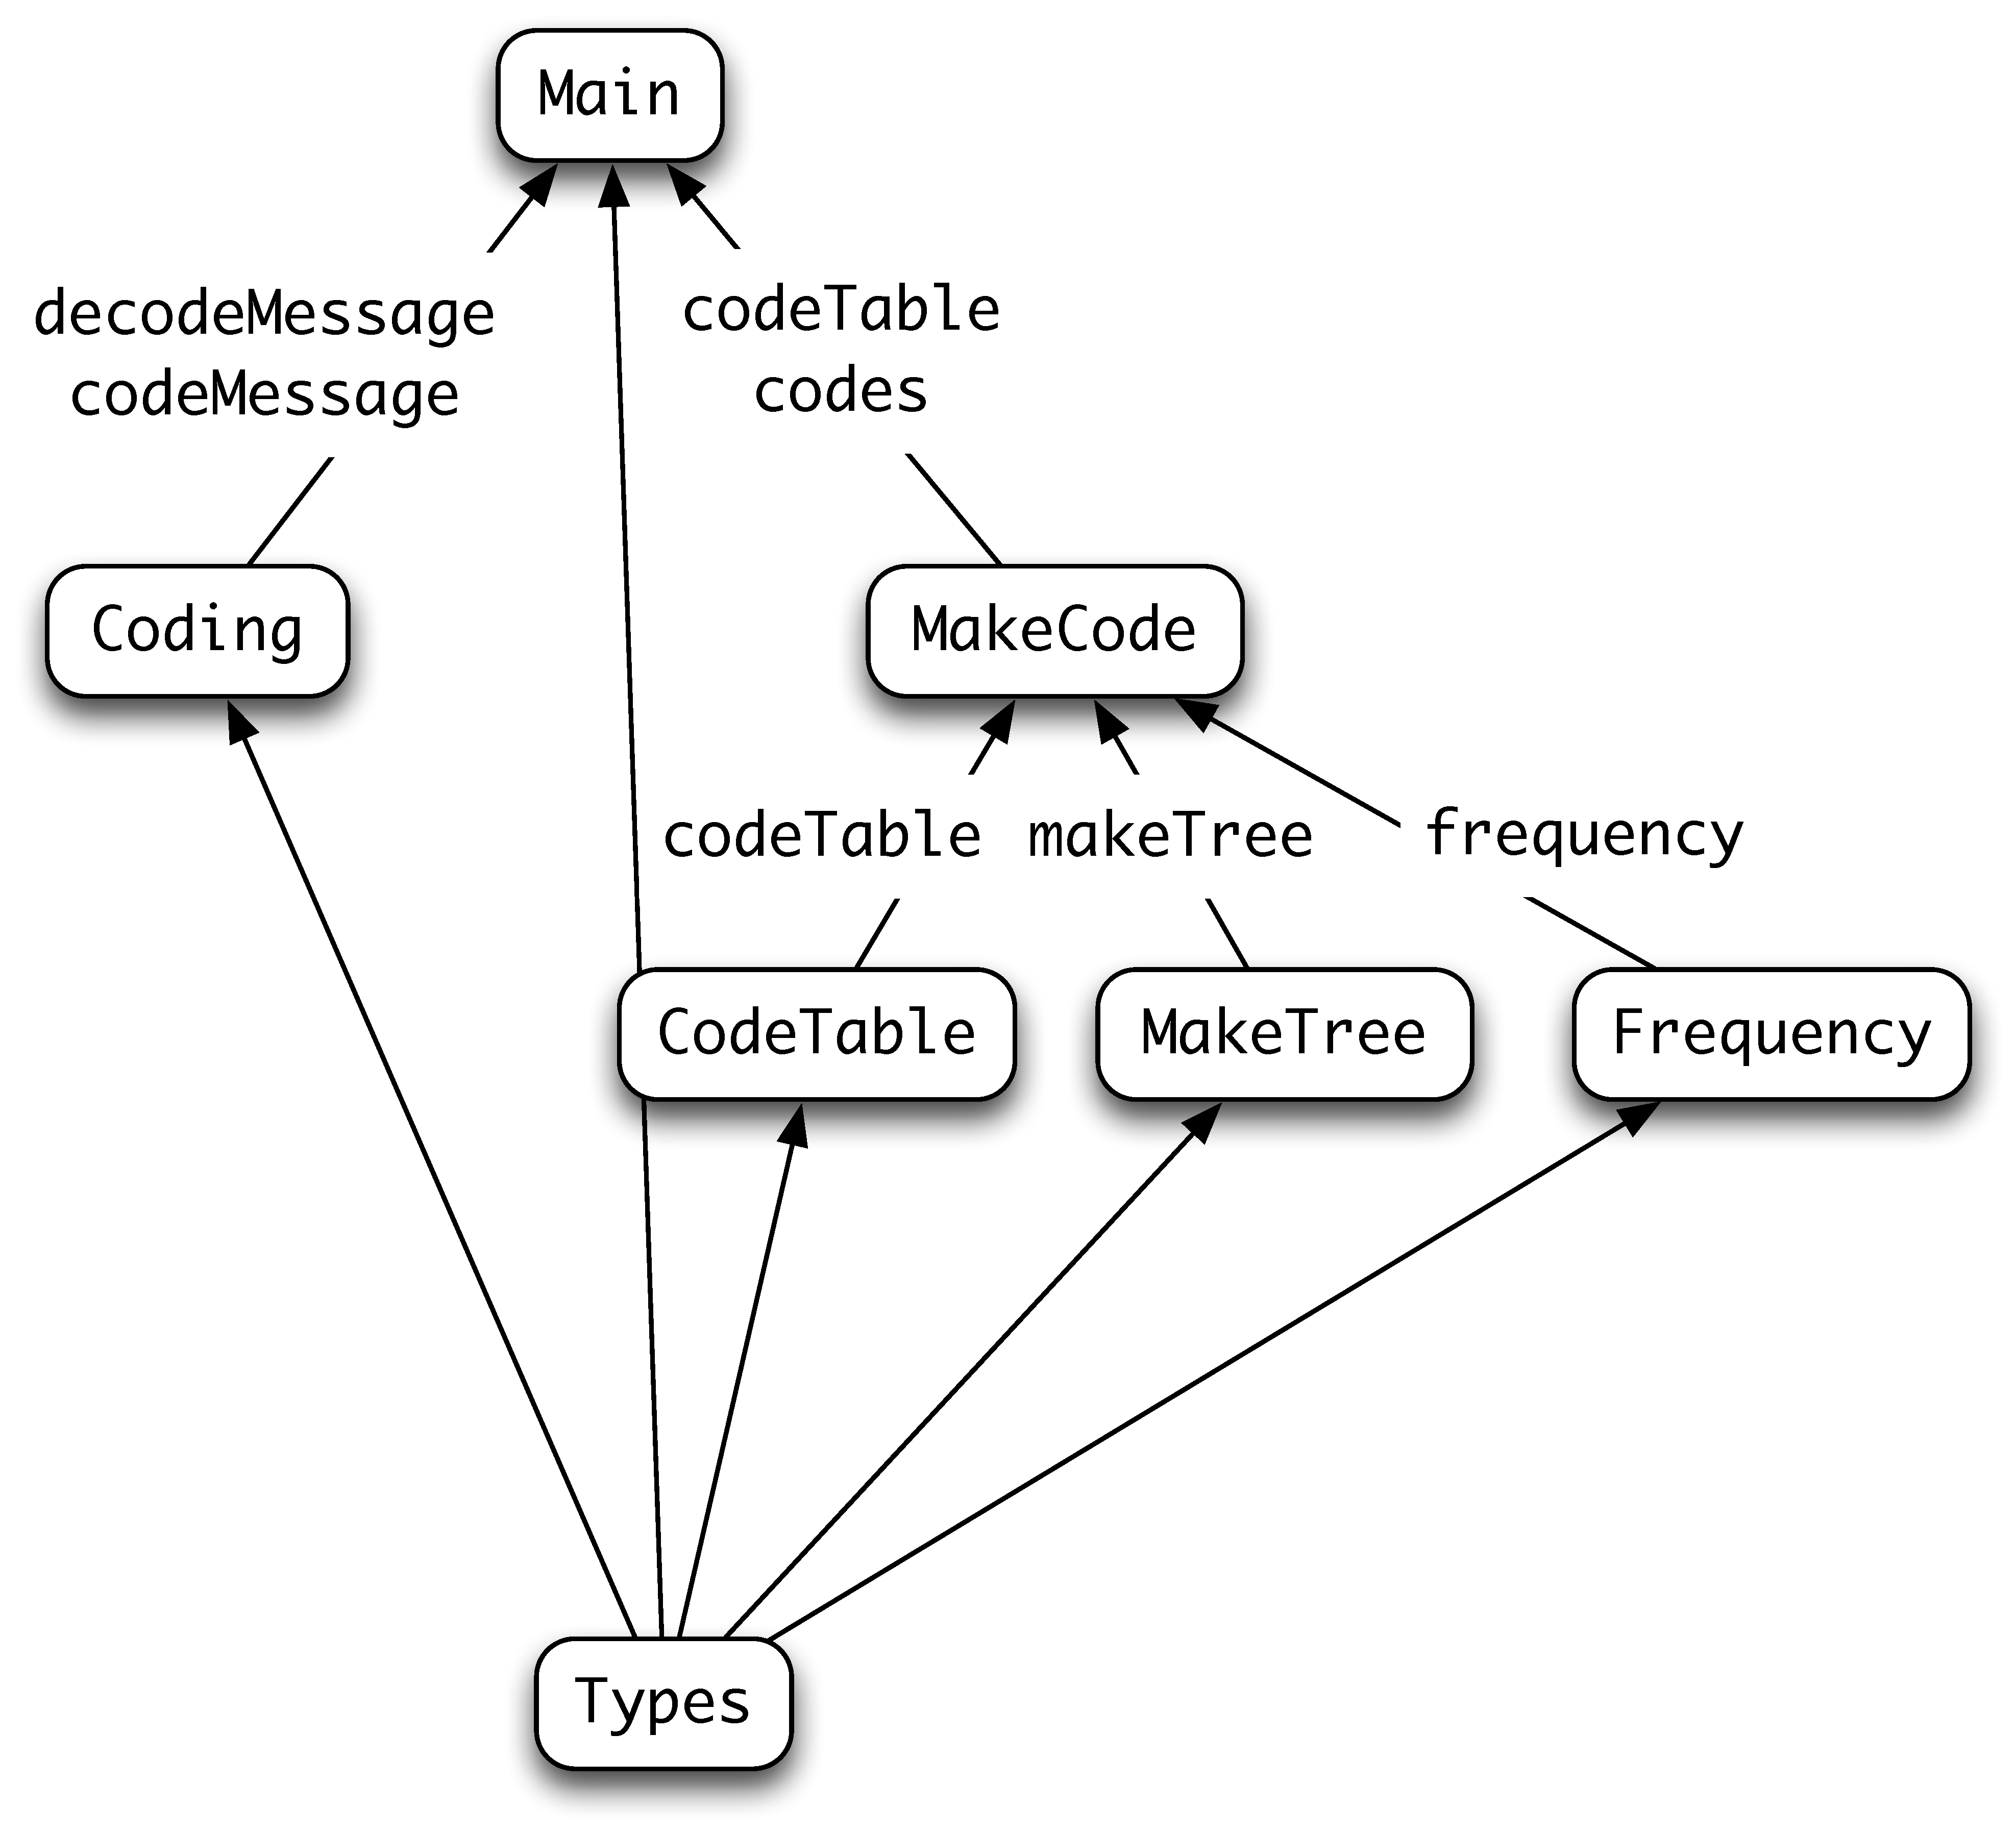
\includegraphics[width=4in]{Pictures/modules.pdf}
\end{center}
\caption{The modules of the Huffman coding system.}
\label{overallMod}
\index{modules!structure diagram}
\end{figure}



\subsection*{The top-level file -- \texttt{Main.hs}}
\minx{Main.hs}

We can now pull all the parts of the system together into a top-level file.
\begin{alltt}
module Main (main) where

import Types    ( Tree(Leaf,Node), Bit(L,R), HCode , Table )
import Coding   ( codeMessage , decodeMessage )
import MakeCode ( codes, codeTable )
\end{alltt}
In this file we can include representative examples, using the major
functions listed in the \texttt{import} statements; the code is illustrated in Figure \ref{mainMod}. 

The
structure of the system is given in Figure \ref{overallMod}. Modules are
represented by boxes, and an arrow from \texttt{A} to \texttt{B} indicates that
\texttt{A.hs} is imported into \texttt{B.hs}. An arrow is marked to indicate the
functions exported by the included module, so that, for example, \texttt{codes}
and \texttt{codeTable} are exported from \texttt{MakeCode.hs} to \texttt{Main.hs}.


If this
coding system were to be used as a component of a larger system, a 
\texttt{module} directive could be used to control which of the four functions and
the types are exported, after the module had been renamed.
It is important to realize that the types will need to
be exported (or be included in the file including \texttt{Main.hs})
if the functions are to be used.

\subsection*{Testing the system}

We can write a top-level test for a system like this, by taking an example string, coding it and then decoding it. This should take us back to the string we started with, and indeed we can see this in the particular example in Figure \ref{mainMod}. It is possible to change this to a QuickCheck property, which checks that coding/decoding is the identity for a whole collection of strings; we leave this as an exercise for the reader.\index{QuickCheck!Huffman codes}

The top-level test corresponds to a \emph{system} test, in that it uses all the functions defined -- implicitly or explicitly -- and checks the overall functionality of the system. It is also possible to write \emph{unit} tests, which check that a particular function or module has the required functionality.

For example, we might look at the module \texttt{Frequency.hs}, and in particular at the functions designed to merge or sort their arguments. A QuickCheck property embodying a unit test for these would include
\begin{alltt}\minx{prop\_mergeSort}
prop_mergeSort :: [Int] -> Bool

prop_mergeSort xs =
    sorted (mergeSort merge xs) 
\end{alltt}
where \texttt{sorted} expresses that its argument is sorted into ascending order and \texttt{merge} will merge two ordered lists in order.



\begin{exercises}

\item
Give a definition of merge sort which uses the built-in ordering `\texttt{<=}'.
What is its type?

\item
Modifying your previous answer if necessary, give a version of merge sort
which removes duplicate entries.

\item
Give a version of merge sort which takes an ordering function as a parameter:
\begin{alltt}
ordering :: a -> a -> Ordering
\end{alltt}
Explain how to implement \texttt{mergeSort freqMerge} using this version of
merge sort, and discuss why you {\em cannot\/} implement \texttt{mergeSort
alphaMerge} this way.

\item
Define the \texttt{insTree} function, used in the definition of \texttt{makeTree}.

\item
Give a calculation of
\begin{alltt}
makeTree  [('b',2),('a',2),('t',3),('e',4)]
\end{alltt}

\item
Define functions
\begin{alltt}
showTree  :: Tree  -> String
showTable :: Table -> String
\end{alltt}
which give printable versions of Huffman trees and code tables. One general
way of printing trees is to use indentation to indicate the structure.
Schematically, this looks like
\begin{alltt}
    left sub tree,  indented by 4 characters
value(s) at Node
    right sub tree, indented by 4 characters
\end{alltt}



\item
Define a QuickCheck property to test coding and decoding: specifically this should code a string and decode it, and compare the result with the original. You may need to restrict the strings over which the test is made.

\item
Define  \texttt{sorted} so that it checks whether its argument is sorted into ascending order and define \texttt{merge} which will merge two ordered lists in order. Using these check whether the property \texttt{prop\_mergeSort ::\ [Int] -> Bool}, defined earlier, holds.

\item
Write QuickCheck unit tests for other functions in \texttt{Frequency.hs} and other modules of the Hufmann coding system.

\item
You may find that it is necessary to restrict the domain over which some properties hold in order for them to QuickCheck successfully: can you re-define the functions involved so that the properties hold for \emph{all} randomly generated inputs.

\item
The correctness property for the Huffman system formulated earlier states that \texttt{decode.code} is the identity. Would you expect that \texttt{code.decode} is the identity: if so, over what domain; if not, can you give a sub-domain over which you wold expect it to hold?


\end{exercises}

\begin{summary}
When writing a program of any size, we need to divide up the work in a
sensible way. The Haskell module system allows one script to be
included in another. At the boundary, it is possible to control exactly which
definitions are exported from one module and imported into another.

We gave a number of guidelines for the design of a program into its
constituent modules. The most important advice is to make each module perform
one clearly defined task, and for only as much information as is needed to be
exported -- the principle of \textbf{information hiding}. This principle 
is extended in the next chapter when we examine abstract
data types.

The design principles were put into practice in the Huffman coding
example. In particular, it was shown for the file \texttt{MakeCode.hs} and
its three sub-modules that design can begin with the design of modules and
their \textbf{interfaces} -- that is the definitions (and their types) which are
exported. Thus the design process starts {\em before\/} any
implementation takes place.
 

\index{Huffman codes|)}

\end{summary}


%\end{document}
